\documentclass{article}

\usepackage{arxiv}

\usepackage[T2A]{fontenc}
\usepackage[utf8]{inputenc}
\usepackage[english, russian]{babel}
% \usepackage{cmap}
\usepackage{url}
\usepackage{booktabs}
\usepackage{nicefrac}
\usepackage{microtype}
\usepackage{lipsum}
\usepackage{graphicx}
\usepackage{epstopdf}
\usepackage{subfig}
\usepackage[square,sort,comma,numbers]{natbib}
\usepackage{doi}
\usepackage{multicol}
\usepackage{multirow}
\usepackage{tabularx}
\usepackage{float}

\usepackage{tikz}
\usetikzlibrary{matrix}

% Algorithms
\usepackage{algpseudocode}
\usepackage{algorithm}

%% Шрифты
\usepackage{euscript} % Шрифт Евклид
\usepackage{mathrsfs} % Красивый матшрифт
\usepackage{extsizes} % Возможность сделать 14-й шрифт
\usepackage{bm}

\usepackage{makecell} % diaghead in a table
\usepackage{amsmath,amsfonts,amssymb,amsthm,mathtools,dsfont}
\usepackage{icomma}
\usepackage[labelfont=bf]{caption}
\usepackage{subfig} % for subfigures
\usepackage{wrapfig}

\newcommand{\bz}{\mathbf{z}}
\newcommand{\bx}{\mathbf{x}}
\newcommand{\by}{\mathbf{y}}
\newcommand{\bv}{\mathbf{v}}
\newcommand{\bw}{\mathbf{w}}
\newcommand{\ba}{\mathbf{a}}
\newcommand{\bb}{\mathbf{b}}
\newcommand{\bp}{\mathbf{p}}
\newcommand{\bq}{\mathbf{q}}
\newcommand{\bt}{\mathbf{t}}
\newcommand{\bu}{\mathbf{u}}
\newcommand{\bs}{\mathbf{s}}
\newcommand{\bT}{\mathbf{T}}
\newcommand{\bX}{\mathbf{X}}
\newcommand{\bZ}{\mathbf{Z}}
\newcommand{\bS}{\mathbf{S}}
\newcommand{\bH}{\mathbf{H}}
\newcommand{\bW}{\mathbf{W}}
\newcommand{\bY}{\mathbf{Y}}
\newcommand{\bU}{\mathbf{U}}
\newcommand{\bQ}{\mathbf{Q}}
\newcommand{\bP}{\mathbf{P}}
\newcommand{\bA}{\mathbf{A}}
\newcommand{\bB}{\mathbf{B}}
\newcommand{\bC}{\mathbf{C}}
\newcommand{\bE}{\mathbf{E}}
\newcommand{\bF}{\mathbf{F}}
\newcommand{\bomega}{\boldsymbol{\omega}}
\newcommand{\btheta}{\boldsymbol{\theta}}
\newcommand{\bgamma}{\boldsymbol{\gamma}}
\newcommand{\bdelta}{\boldsymbol{\delta}}
\newcommand{\bPsi}{\boldsymbol{\Psi}}
\newcommand{\bpsi}{\boldsymbol{\psi}}
\newcommand{\bxi}{\boldsymbol{\xi}}
\newcommand{\bchi}{\boldsymbol{\chi}}
\newcommand{\bzeta}{\boldsymbol{\zeta}}
\newcommand{\blambda}{\boldsymbol{\lambda}}
\newcommand{\beps}{\boldsymbol{\varepsilon}}
\newcommand{\bZeta}{\boldsymbol{Z}}
% mathcal
\newcommand{\cX}{\mathcal{X}}
\newcommand{\cY}{\mathcal{Y}}
\newcommand{\cW}{\mathcal{W}}

\newcommand{\dH}{\mathds{H}}
\newcommand{\dR}{\mathds{R}}
% transpose
\newcommand{\T}{^{\mathsf{T}}}

% \renewcommand{\shorttitle}{\textit{arXiv} Шаблон}
\renewcommand{\epsilon}{\ensuremath{\varepsilon}}
\renewcommand{\phi}{\ensuremath{\varphi}}
\renewcommand{\kappa}{\ensuremath{\varkappa}}
\renewcommand{\le}{\ensuremath{\leqslant}}
\renewcommand{\leq}{\ensuremath{\leqslant}}
\renewcommand{\ge}{\ensuremath{\geqslant}}
\renewcommand{\geq}{\ensuremath{\geqslant}}
\renewcommand{\emptyset}{\varnothing}

\DeclareMathOperator*{\argmax}{arg\,max}  % in your preamble
\DeclareMathOperator*{\argmin}{arg\,min}  % in your preamble 

\usepackage{hyperref}
% \usepackage[usenames,dvipsnames,svgnames,table,rgb]{xcolor}

\hypersetup{
	unicode=true,
	colorlinks=true,
	linkcolor=black,        % внутренние ссылки
	citecolor=blue,         % на библиографию
	filecolor=magenta,      % на файлы
	urlcolor=blue           % на URL
}

\graphicspath{{./figures}}

\usepackage{enumitem} % Для модификаций перечневых окружений

\theoremstyle{definition} % "Определение"
\newtheorem{definition}{Опр.}[section]

\usepackage{etoolbox}

\makeatletter
\expandafter\patchcmd\csname\string\algorithmic\endcsname{\itemsep\z@}{\itemsep=1.5mm}{}{}
\makeatother

\newcommand{\myfigref}[2]{~\ref{#1}.\subref{#2}}% <---- a new macro for referring to a subfigure

\begin{document}
\maketitle

\begin{abstract}

The problem of reconstructing the dependence between fMRI sensor readings 
and human perception of the external world is investigated. 
The dependence between the sequence of fMRI images and the video sequence 
viewed by a person is analyzed. Based on the dependence study, a method for 
approximating fMRI readings from the viewed video sequence is proposed. 
The method is constructed under the assumption of the presence of a time 
invariant hemodynamic response time dependence of blood oxygen level. 
A linear model is independently constructed for each voxel of the fMRI image.  
The assumption of markovality of the fMRI image sequence is used. 
To analyze the proposed method, a computational experiment is performed 
on a sample obtained during tomographic examination of a large number of subjects. 
The dependence of the method performance quality on the hemodynamic response 
time is analyzed on the experimental data. Hypotheses about invariance of 
model weights with respect to a person and correctness of the constructed 
method are tested.

\end{abstract}


\keywords{neuroimaging \and fMRI \and video sequences \and correlation analysis
\and hypothesis testing \and linear model \and forecasting}

\section{Introduction}

A set of techniques that visualize the structure and function of the human brain,
is called \textit{neurovisualization}. Neuroimaging \citep{puras2014neurovisualization} techniques such as ECG, CT, MRI, and fMRI,
are used to study the brain and to detect disease and mental disorders.

\textit{Functional magnetic resonance imaging}, or \textit{fMRI}.
is a type of MRI based on changes in blood flow,
caused by neural activity in the brain \citep{Glover2011}.
These changes don't occur instantaneously, but with a delay,
which is 4--8 seconds \citep{Bandettini1992}.
It's because it takes the vascular system a long time to respond
to the brain's need for glucose \citep{Ogawa1990, LEBIHAN1995231, Logothetis2003}. 

In fMRI imaging, sequences of
echoplanar imaging (EPI) \citep{Connelly1993, Kwong1992, Ogawa1992}.
Processing of areas with varying signal intensity depending on the method of activation, the type of artifact.
depending on the method of activation, the type of artifacts and duration
is carried out using special methods and programs 
\citep{Bandettini1992, BAUDENDISTEL1995701, COX1996162}.
The processed results are formalized as activation maps,
which are combined with the localization of anatomical structures
of the cerebral cortex.

The fMRI method plays a major role in neuroimaging, but has some important limitations.
The works of \citep{menon1999spatial, logothetis2008we} discuss the
temporal and spatial resolutions of fMRI. Temporal resolution is a significant
disadvantage of this method. Another disadvantage of fMRI~--- the inevitable noise,
associated with movement of the object in the scanner, human heartbeat and respiration, thermal
fluctuations of the device itself, etc. In the work \citep{1804.10167} proposed methods of
graph-based methods for suppressing the above-mentioned noises and demonstrates their effectiveness in the task of
epilepsy and depression detection.

In fMRI, the subject is given a variety of test tasks and external stimuli that induce activation of specific
external stimuli are applied, causing activation of certain
localized areas of the brain that are responsible for performing
of the brain responsible for its functions.
Various test tasks are applied: movements of fingers and limbs 
\citep{Roux1998, Papke1999}, image finding and examination
of a chessboard \citep{Engel1994, Schneider1994},
listening to non-specific noises, single words or coherent text \citep{Binder1994, Dymarkowski1998}.
Changes in human brain activity during fMRI examinations
could also be caused by viewing the video of \citep{decety1997brain},
which is the subject of this paper.

The most well-known video processing methods are based on 3D convolutions \citep{tran2015learning}.
The difference between 3D and 2D convolutions is the simultaneous work with the spatial and temporal part of the information.
of information. A significant disadvantage of these methods is the strong increase in the number of model parameters and the
large computational costs. One of the most modern and improving architectures of
neural networks for image processing is the ResNet~\citep{he2015deep} residual neural network.
It allows training deep neural networks (up to 152 layers) with high accuracy,
overcoming the problem of gradient fading that arises when training deep networks.

The real work is devoted to recovering the dependence between fMRI images and video sequences.
The assumption that such a dependence exists is used.
In addition, it is assumed that there is a constant time delay between the image and the video sequence
\citep{Logothetis2003}.
The dependence of the fMRI image on one image and the previous image is tested.
The delay time acts as a hyperparameter of the model.
Based on the dependence analysis, a method is proposed to approximate the fMRI readings from the
the viewed video sequence.

According to a study \citep{anderson2006}, when patients undergo fMRI,
viewing a video sequence activates a specific cortical network. This network includes
including the occipital lobe and frontal regions. This network is located
predominantly in the right hemisphere. In this paper, we're considering an approach
that uses these parts of the brain to analyze latency time.

The data on which the dependence hypothesis is tested and the demonstration of the work of the constructed method
 are presented in the paper \citep{Berezutskaya2022}.
This data set was obtained from examination of a group of 63 subjects. Thirty of them underwent fMRI examination.
They were asked to perform the same task~--- viewing a short audiovisual movie.
For it, annotations were generated in the paper under review, containing, among other things, information about the time of appearance and disappearance of
of individual words, objects and characters. The methods of audio and video annotation are described in detail in the
\citep{boersma2018praat} and \citep{Berezutskaya2020}.

\section{Problem statement}

Frame rate $\nu \in \mathbb{R}$ and duration $t \in \mathbb{R}$ of the video sequence are set.
The video sequence is set as
\begin{equation}
	\label{eq1}
	\bP = [\bp_1, \ldots, \bp_{\nu t}], \quad\
	\bp_{\ell} \in \mathbb{R}^{W \times H \times C},
\end{equation}
with width, height and number of image channels $W, H$ and $C$, respectively.

Let us denote the frequency of fMRI images by $\mu \in \mathbb{R}$. We set the sequence of images
\begin{equation}
	\label{eq2}
	\bS = [\bs_1, \ldots, \bs_{\mu t}], \quad\
	\bs_{\ell} \in \mathbb{R}^{X \times Y \times Z},
\end{equation}
where $X, Y$, and $Z$~--- the dimensions of the voxel image.

The problem is to construct a mapping that accounts for the $\Delta t$ delay between the fMRI image and the video sequence, as well as previous tomographic readings.
fMRI image and the video sequence, as well as previous tomographic readings. Formally, it is necessary to
find such a mapping $\mathbf{g}$ that
\begin{equation}
	\label{eq3}
	\mathbf{g}(\bp_1, \ldots, \bp_{k_{\ell} - \nu \Delta t}; \bs_1, \ldots, \bs_{\ell-1}) = \bs_{\ell},
	\ \ell = 1, \ldots, \mu t,
\end{equation}
where for the $\ell$-th fMRI image the number of the corresponding image $k_{\ell}$ is determined by the formula
\begin{equation}
	\label{eq4}
	k_{\ell} = \dfrac{\ell \cdot \nu}{\mu}.
\end{equation}

\section{Proposed forecasting method}

The scheme of the proposed fMRI image reconstruction method is shown in Figure~\ref{fig:scheme}. 

\begin{figure}[h!]
	\centering
	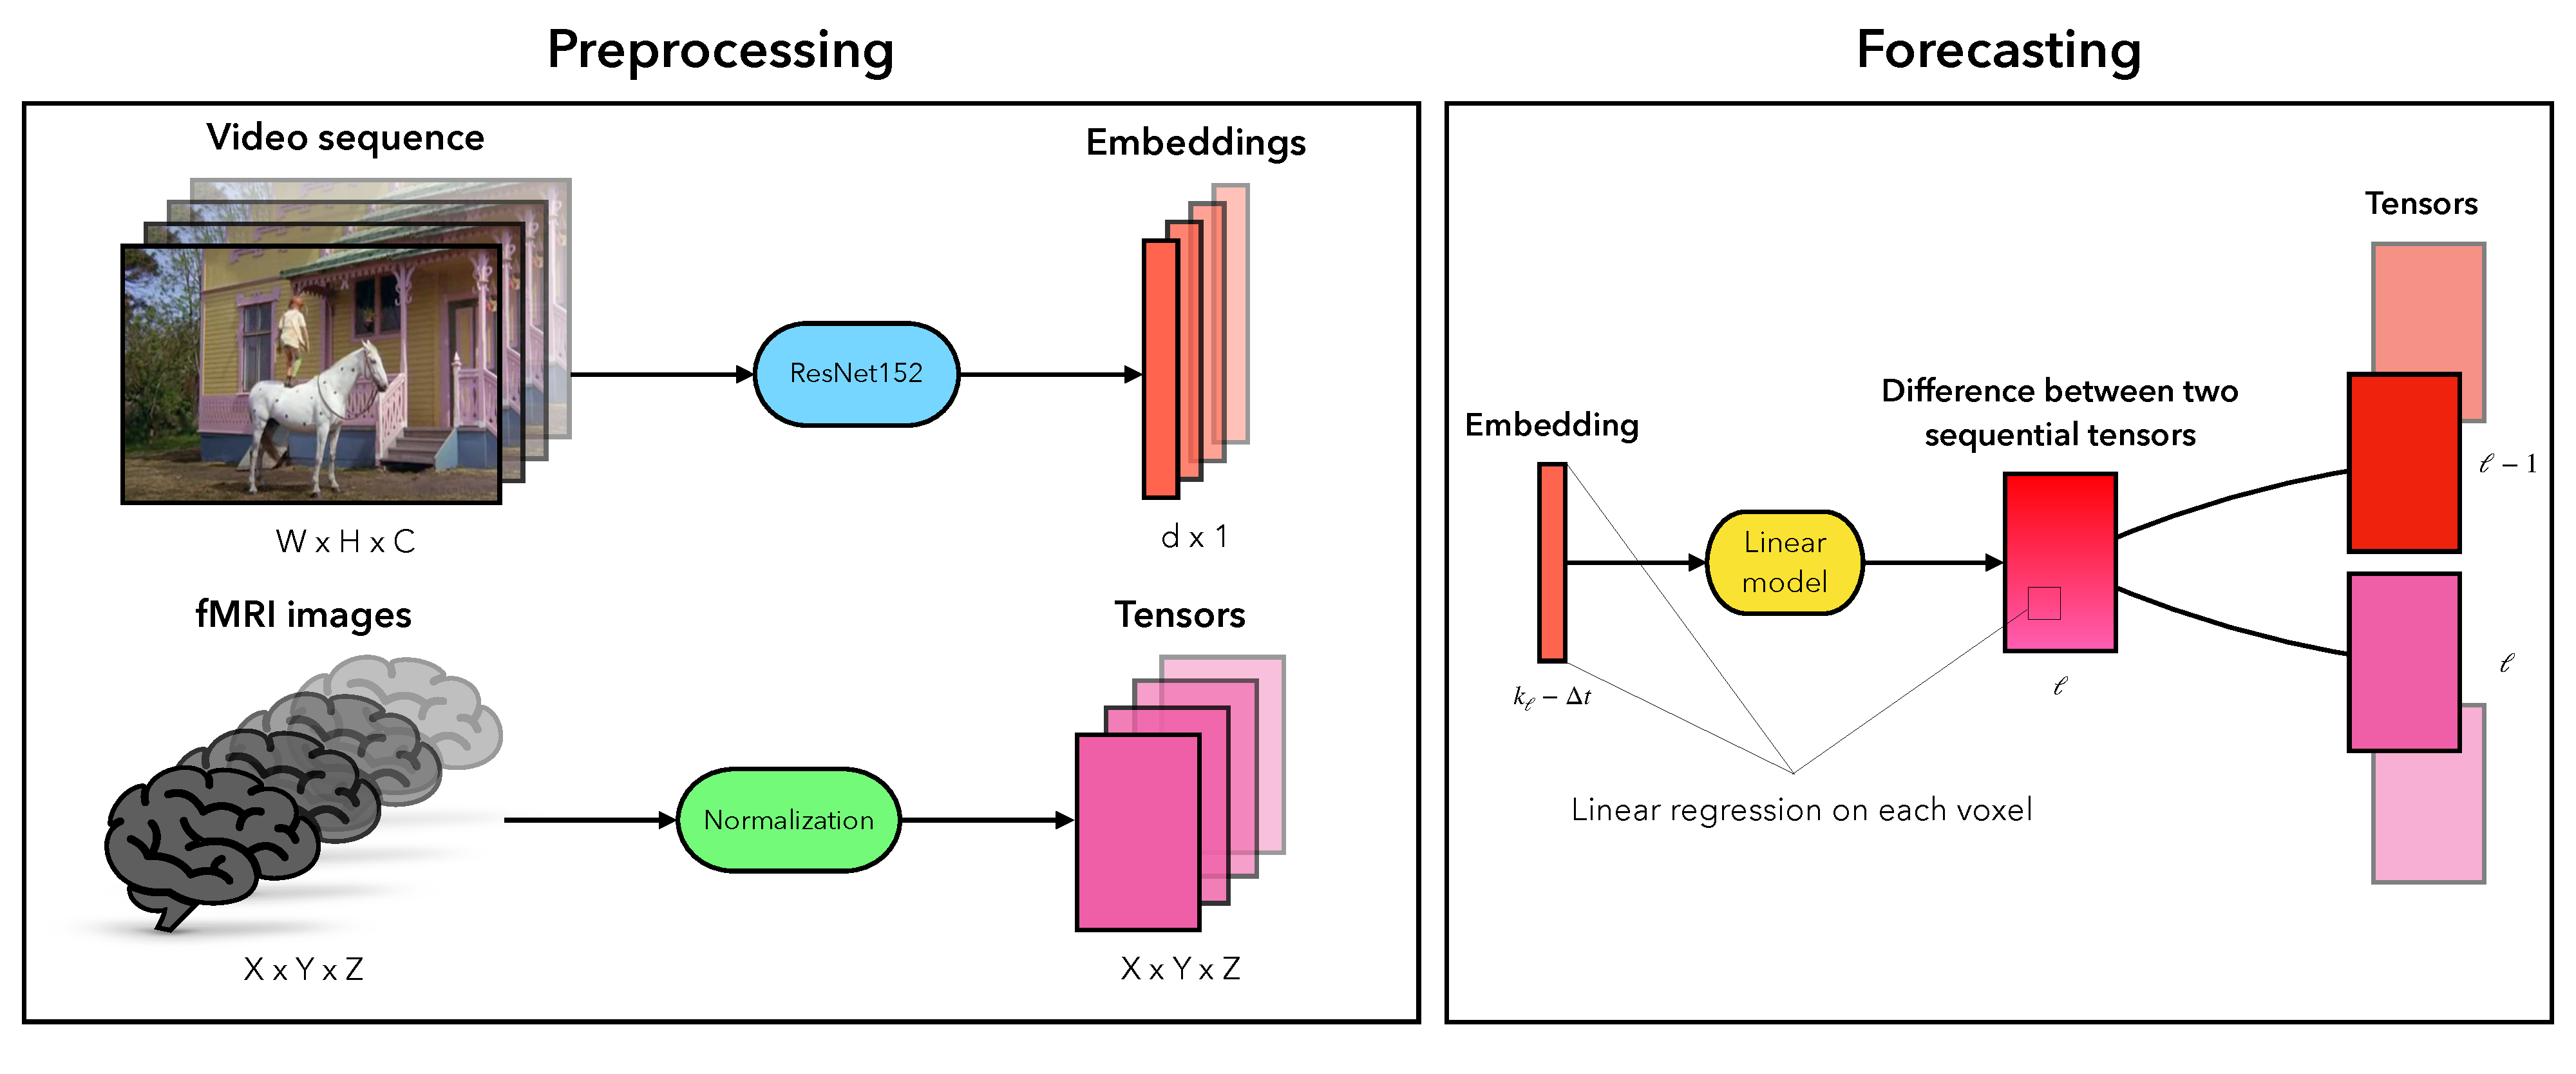
\includegraphics[width=\textwidth]{scheme.pdf}
	\caption{Method scheme}
	\label{fig:scheme}
\end{figure}

We denote the fMRI image as $\bs_{\ell} = [v^{\ell}_{ijk}] \in \mathbb{R}^{X \times Y \times Z}$,
where $v^{\ell}_{ijk} \in \mathbb{R}_+$~--- value of the corresponding voxel.
In order to reduce the running time of the method, we propose to use compression of fMRI images by dimensionality reduction.
Compression by a factor of 2 is represented in the form of a mapping
\[\bm{\chi}: \mathbb{R}^{X \times Y \times Z} \to \mathbb{R}^{X/2 \times Y/2 \times Z/2}.\]
A compression of $2^k$ times is obtained by applying $\bm{\chi}$ successively $k$ times. 
In the following, for simplicity, we keep the notation of image dimensions $X \times Y \times Z$.

Suppose that the Markov property is satisfied for the sequence of snapshots,
i.e., each snapshot depends only on one image and the previous snapshot.
Then the corresponding mapping is written in the form
\begin{equation}
	\label{eq5}
	\mathbf{g}(\bp_{k_{\ell} - \nu \Delta t}) = \bs_{\ell} - \bs_{\ell-1} = \bdelta_{\ell}, \ \ell = 2, \ldots, \mu t.
\end{equation}
where $\bdelta_{\ell} = [v^{\ell}_{ijk} - v^{\ell-1}_{ijk}] = [\delta^{\ell}_{ijk}] \in \mathbb{R}^{X \times Y \times Z}$~--- the difference between two consecutive snapshots.

Mapping $\mathbf{g}: \mathbf{P} \to \mathbf{S}$ is represented as a composite of the other two:
\[ \mathbf{g} = \bm{\varphi} \circ \bm{\psi}, \]
\vspace{-0.5cm}
\begin{align*}
	 & \bm{\psi}: \mathbf{P} \to \mathbb{R}^d
	\text{~--- image vectorization,}        \\
	 & \bm{\varphi}: \mathbb{R}^d \to \mathbf{S}
	\text{~--- restorable mapping.}
\end{align*}

For each image from the video sequence, we have an embedding vector of dimension $d$:
\[ \bx_{\ell} = [x^{\ell}_1, \ldots, x^{\ell}_{d}]\T \in \mathbb{R}^{d}, \ {\ell} = 1, \ldots, \nu t. \]
The ResNet152 neural network architecture without the last linear layer is used.

Given \eqref{eq4}, the total number of pairs (image, snapshot)
is $N = \mu (t - \Delta t)$. Thus, for each voxel a sample is given
\[ \mathfrak{D}_{ijk} = \{(\bx_{\ell}, \delta^{\ell}_{ijk}) \ | \ {\ell} = 2, \ldots, N \}. \]

The regression task is set
\begin{equation}
	\label{eq6}
	y_{ijk}: \mathbb{R}^{d} \to \mathbb{R}.
\end{equation}

A linear model is used with a vector of parameters
\[ \bw_{ijk} = [w^{ijk}_1, \ldots, w^{ijk}_{d}]\T \in \mathbb{R}^{d}: \]
\begin{equation}
	\label{eq7}
	f_{ijk}(\bx, \bw_{ijk}) = \langle \bx, \bw_{ijk} \rangle.
\end{equation}

For the model $f_{ijk}$ with its corresponding parameter vector $\bw_{ijk} \in \mathbb{R}^{d}$
define a quadratic loss function with $L_2$ regularization:
\begin{equation}
	\label{eq8}
	\mathcal{L}_{ijk}(\bw_{ijk}) = \sum\limits_{\ell = 2}^{N} \big(f_{ijk}(\bx_{\ell}, \bw_{ijk}) - \delta^{\ell}_{ijk}\big)^2 + \alpha \| \bw_{ijk} \|_2^2,
\end{equation}
where $\alpha \in \mathbb{R}$~--- regularization coefficient.

It is required to find the parameters that give a minimum to the loss functional $\mathcal{L}_{ijk}(\bw_{ijk})$
for given hyperparameters $\Delta t$ and $\alpha$:
\begin{equation}
	\label{eq9}
	\hat{\bw}_{ijk} = \argmin_{\bw_{ijk}} \mathcal{L}_{ijk}(\bw_{ijk}).
\end{equation}

The minimum of the loss function is found by the least squares method. Let's define the matrix of objects-features
\begin{equation}
	\label{eq10}
	\bX = [\bx_2, \ldots, \bx_N]\T = [x^i_j] \in \mathbb{R}^{(N-1) \times d}
\end{equation}
and a vector whose components are the differences of values of the same voxel in different images,
\begin{equation}
	\label{eq11}
	\mathbf{\Delta}_{ijk} = [\delta^2_{ijk}, \ldots, \delta^N_{ijk}]\T \in \mathbb{R}^{N-1}.
\end{equation}

The solution is written in the form
\begin{equation}
	\label{eq12}
	\hat{\bw}_{ijk} = (\bX\T \bX + \alpha \mathbf{I})^{-1} \bX\T \mathbf{\Delta}_{ijk}.
\end{equation}

Let us obtain a formula for reconstructed fMRI images. Let's introduce a matrix of weights
\begin{equation}
	\label{eq13}
	\hat{\bW} = [\hat{\bw}_1, \ldots, \hat{\bw}_{XYZ}]\T = [\hat{w}^i_j] \in \mathbb{R}^{XYZ \times d}.
\end{equation}

Let's introduce for tensors $\bs_{\ell}, \bdelta_{\ell} \in \mathbb{R}^{X \times Y \times Z}$ vectors
\[ \bs_{\ell}^{R} = [ v^{\ell}_1, \ldots, v^{\ell}_{XYZ} ]\T,\
	\bdelta_{\ell}^{R} = [ \delta^{\ell}_1, \ldots, \delta^{\ell}_{XYZ} ]\T \in \mathbb{R}^{XYZ}. \]

Then the vector of the forecasted image is found by the formula
\begin{equation}
	\label{eq14}
	\hat{\bs}_{\ell}^{R} = \bs_{\ell-1}^{R} + \hat{\bdelta}_{\ell}^{R} = \bs_{\ell-1}^{R} + \hat{\mathbf{W}} \mathbf{x}_{\ell}.
\end{equation}

\section{Numerical experiment}

To analyze the performance of the proposed method and test the hypotheses
a computational experiment was carried out.

The sample presented in \citep{Berezutskaya2022} was used as data.
The dataset contains the results of examination of 63 subjects.
For thirty of them fMRI readings are known.
There are 16 males and 14 females, ranging in age from 7 to 47 years.
The mean age of the subjects~--- 22 years.

Characteristics of the sample: duration of examination,
frame rates of fMRI video sequences and images, and their dimensions are summarized in Table~\ref{table:sample}.

\begin{table}[h!]
	\centering
	\caption{Dataset Description}
	\begin{tabular}{|c|c|c|}
		\hline
		Name                       & Notation & Value             \\
		\hline \hline
		Duration of examination & $t$         & 390 s                \\ \hline
		Video frame rate           & $\nu$       & 25 Hz   \\ \hline
		fMRI frame rate           & $\mu$       & 1.64 Hz \\ \hline
		Video dimensions        & $W, H, C$   & 640, 480, 3          \\ \hline
		fMRI dimensions             & $X, Y, Z$   & 40, 64, 64           \\ \hline
	\end{tabular}
	\label{table:sample}
\end{table}

The sample was divided into training and test samples in the ratio of 70\% and 30\%, respectively.
The quality criterion for fMRI image reconstruction is MSE~--- the sum of squares of deviations
between the true and reconstructed images, averaged over all voxels of each image.
from the test sample.

To reduce the running time of the algorithm, the fMRI image is precompressed
using MaxPool3D layer. Compression ratios of 1, 2, 4 and 8 are considered.
The voxel values are normalized to $[0; 1]$ by the MinMaxScale procedure.

Table~\ref{table:pc} summarizes the specifications of the computer on which the computational experiment was
on which the computational experiment was performed.

\begin{table}[h!]
	\centering
	\caption{PC Specification}
	\begin{tabular}{|c|c|}
		\hline
		Element & Description \\
		\hline \hline
		CPU & Intel Core i7-7700 3.6 GHz \\ \hline
		GPU & NVIDIA GeForce GTX 1060 3 GB \\ \hline
		RAM & 16 GB 2400 MHz \\ \hline
		Hard Drive & M.2 SSD \\ \hline
		OS & Windows 10 \\ \hline
	\end{tabular}
	\label{table:pc}
\end{table}

\paragraph*{Method performance.}

Figure~\ref*{fig:example} shows slices of the true and reconstructed images from the test sample.
Figure\myfigref{fig:example}{fig:example-c} shows the difference between them.
To demonstrate the performance of the algorithm, the 7th subject was selected, $\Delta t = 5 \text{s}$, compression factor 1, regularization factor
$\alpha = 1000$. The 20th slice along the first coordinate of the 37th image in the sequence was considered.
Since the voxel values are normalized to the segment $[0; 1]$, an error of the order of $10^{-3}$
indicates a fairly accurate prediction.

\begin{figure}[h!]
	\centering
	\subfloat[Test]{\label{fig:example-a}{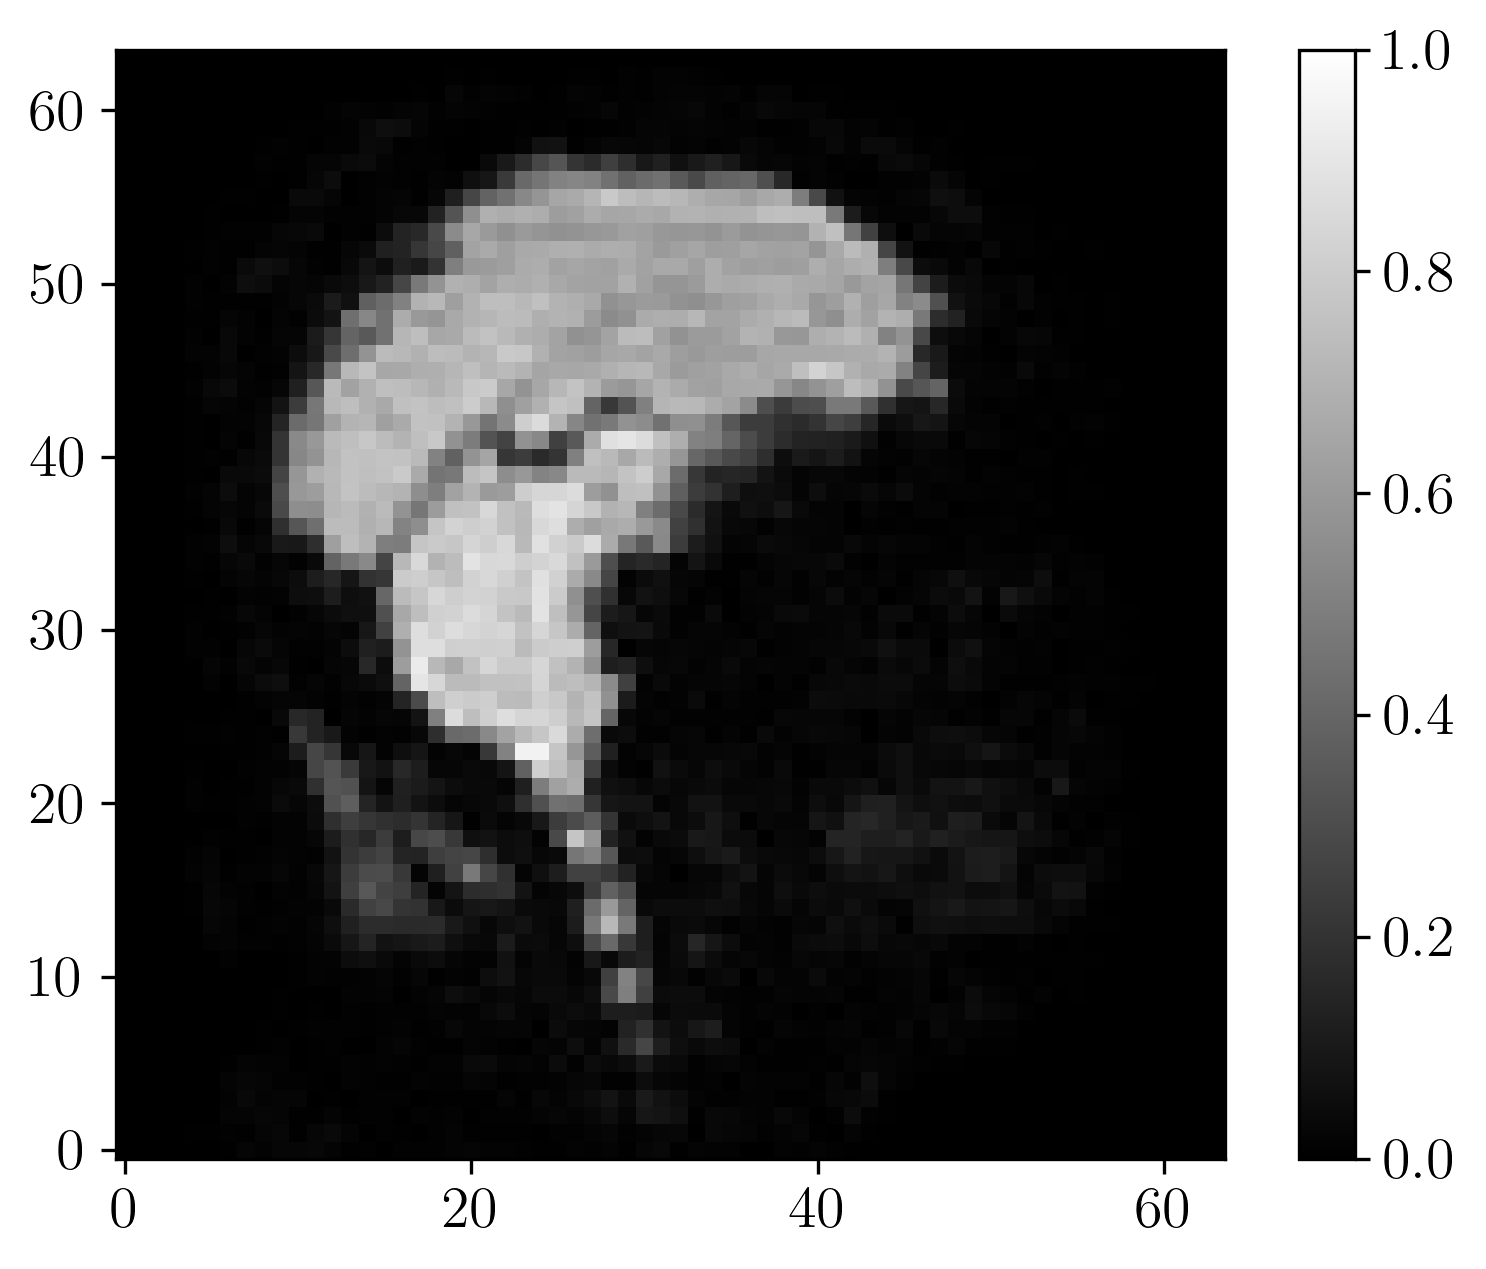
\includegraphics[width=0.33\textwidth]{sub-07-5-1-1000-37-20-_-_-test.png}}}
	\hfill
	\subfloat[Predicted]{\label{fig:example-b}{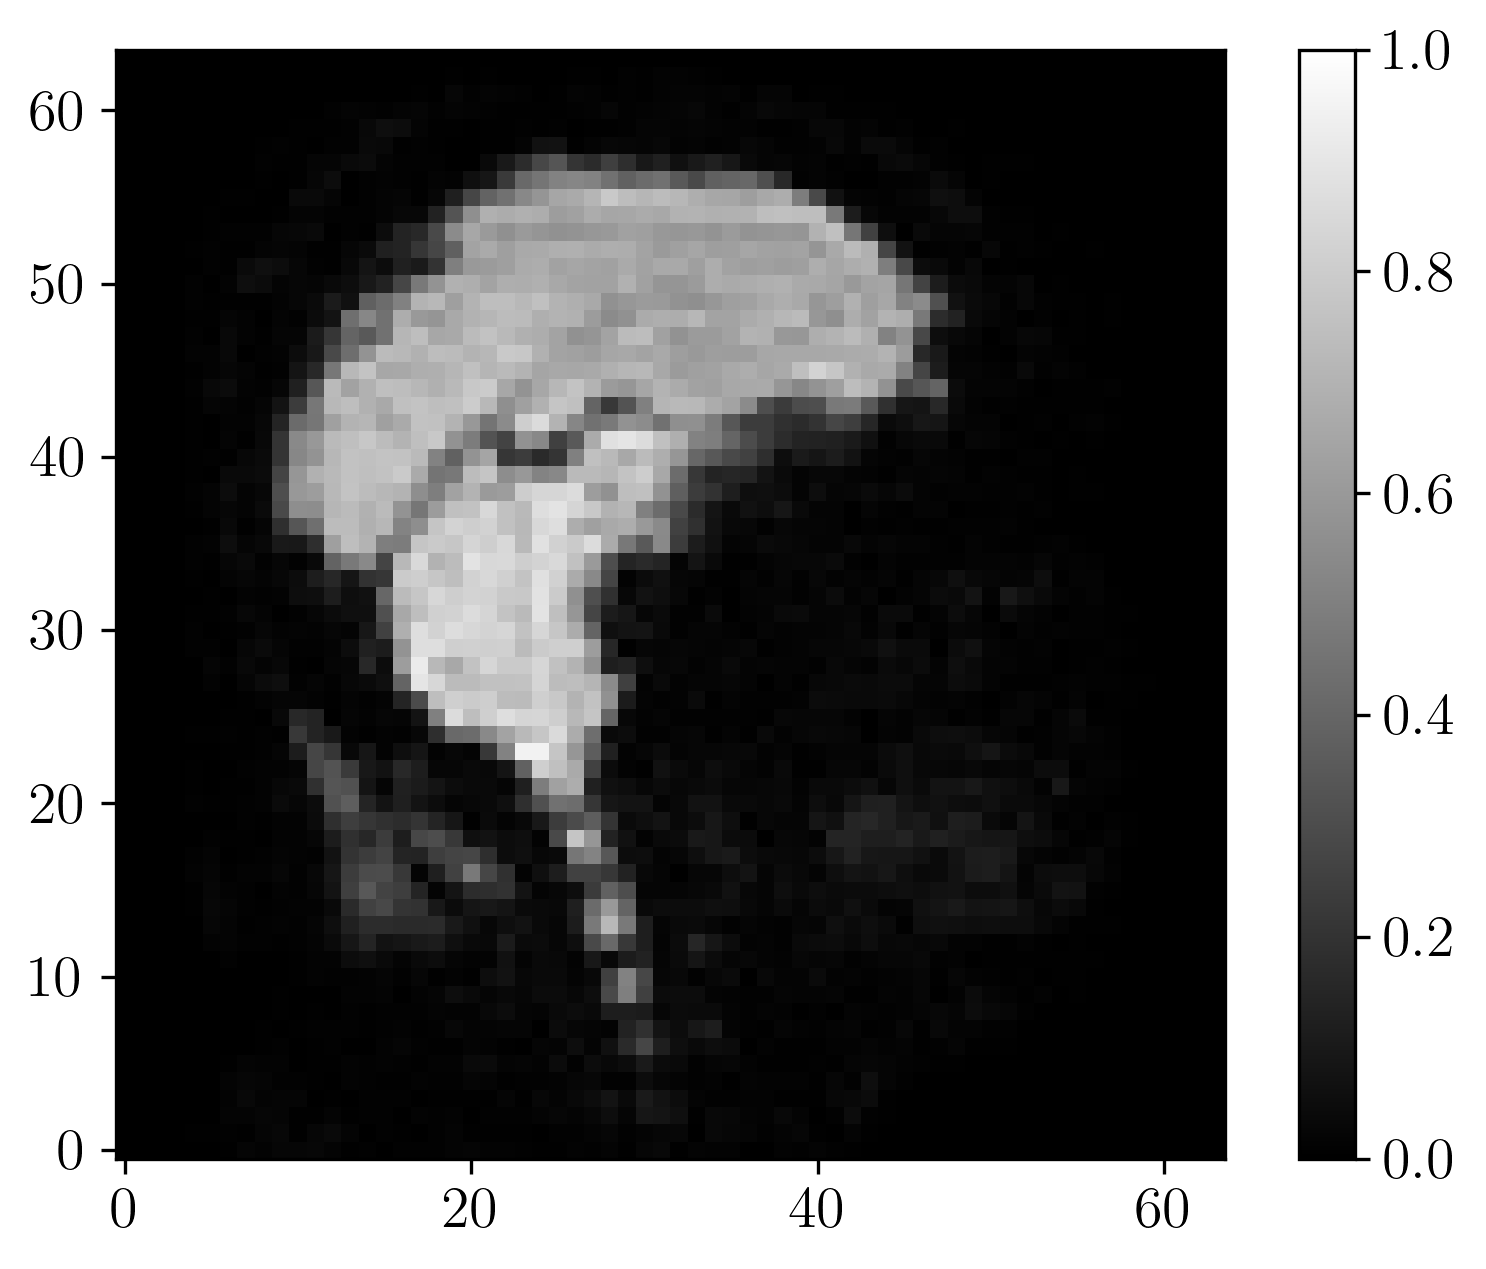
\includegraphics[width=0.33\textwidth]{sub-07-5-1-1000-37-20-_-_-predicted.png}}}
	\hfill
	\subfloat[Difference]{\label{fig:example-c}{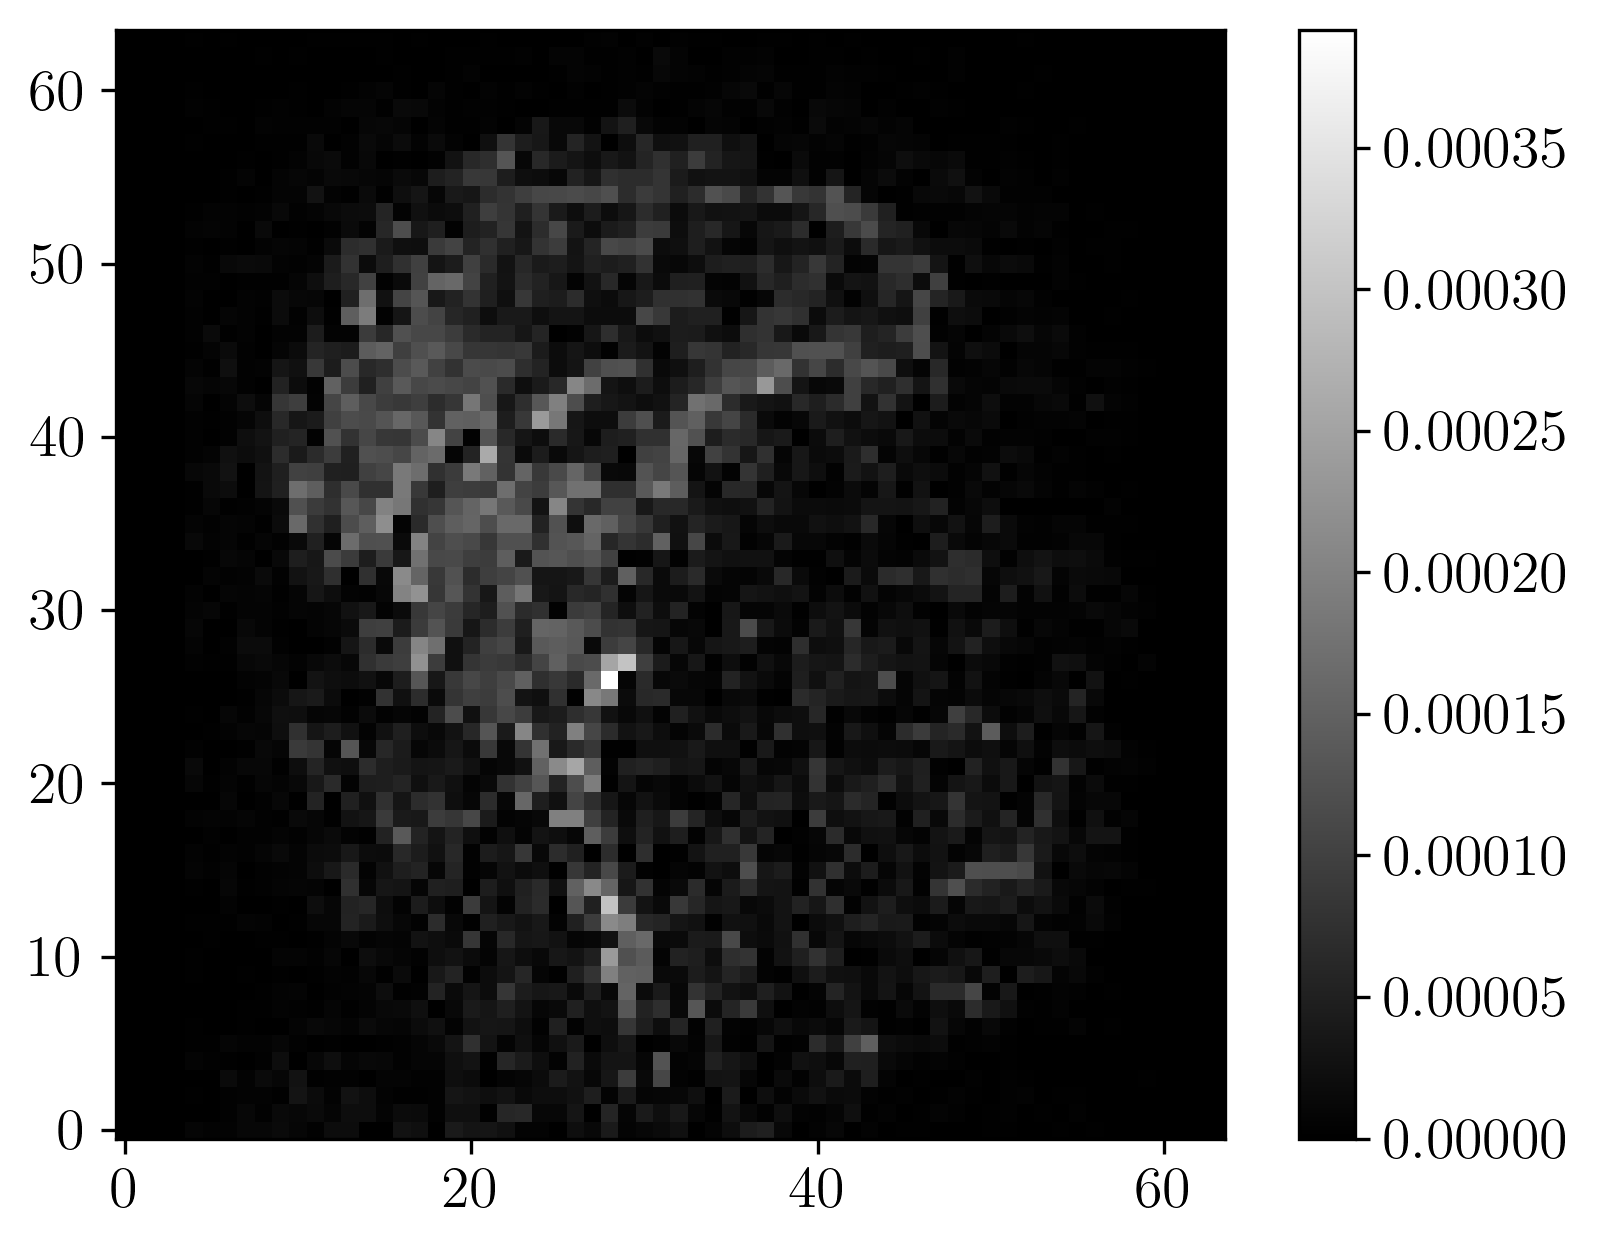
\includegraphics[width=0.33\textwidth]{sub-07-5-1-1000-37-20-_-_-difference.png}}}
	\caption{Slices of fMRI images from the test sample}
	\label{fig:example}
\end{figure}

\paragraph*{Delay time analysis.}

The dependence of recovery quality on delay time was investigated.
The 47th subject and 4x compression were chosen for the example.
The left graph in Figure~\ref{fig:mse-dt} shows the dependence of the MSE metric
on the delay time $\Delta t$.
The study confirms that the most active part of the brain is the most active part of the brain 
in this examination~--- the occipital lobe.
The other parts contribute noise to the considered dependence.
In the present work, the above-mentioned region is localized, 
as shown in Figure~\ref{fig:local}.
To localize the region, the lower third and the right two thirds of the volumetric
of the tomographic image.
The area highlighted in red is the area that contains the 3\% 
of the most variable voxels in the occipital lobe.
For this purpose, all voxels of the localized area were ordered by 
descending order of the total absolute change in values.
Then 3\% of voxels with the largest changes were selected.
The MSE metric was recalculated exactly on this part of the image.
The corresponding graph is shown on the right side of Figure~\ref{fig:mse-dt}.
There is a more distinct minimum at $\Delta t \approx 5$ seconds.

\begin{figure}[h!]
	\centering
	\subfloat[True]{\label{fig:local-a}{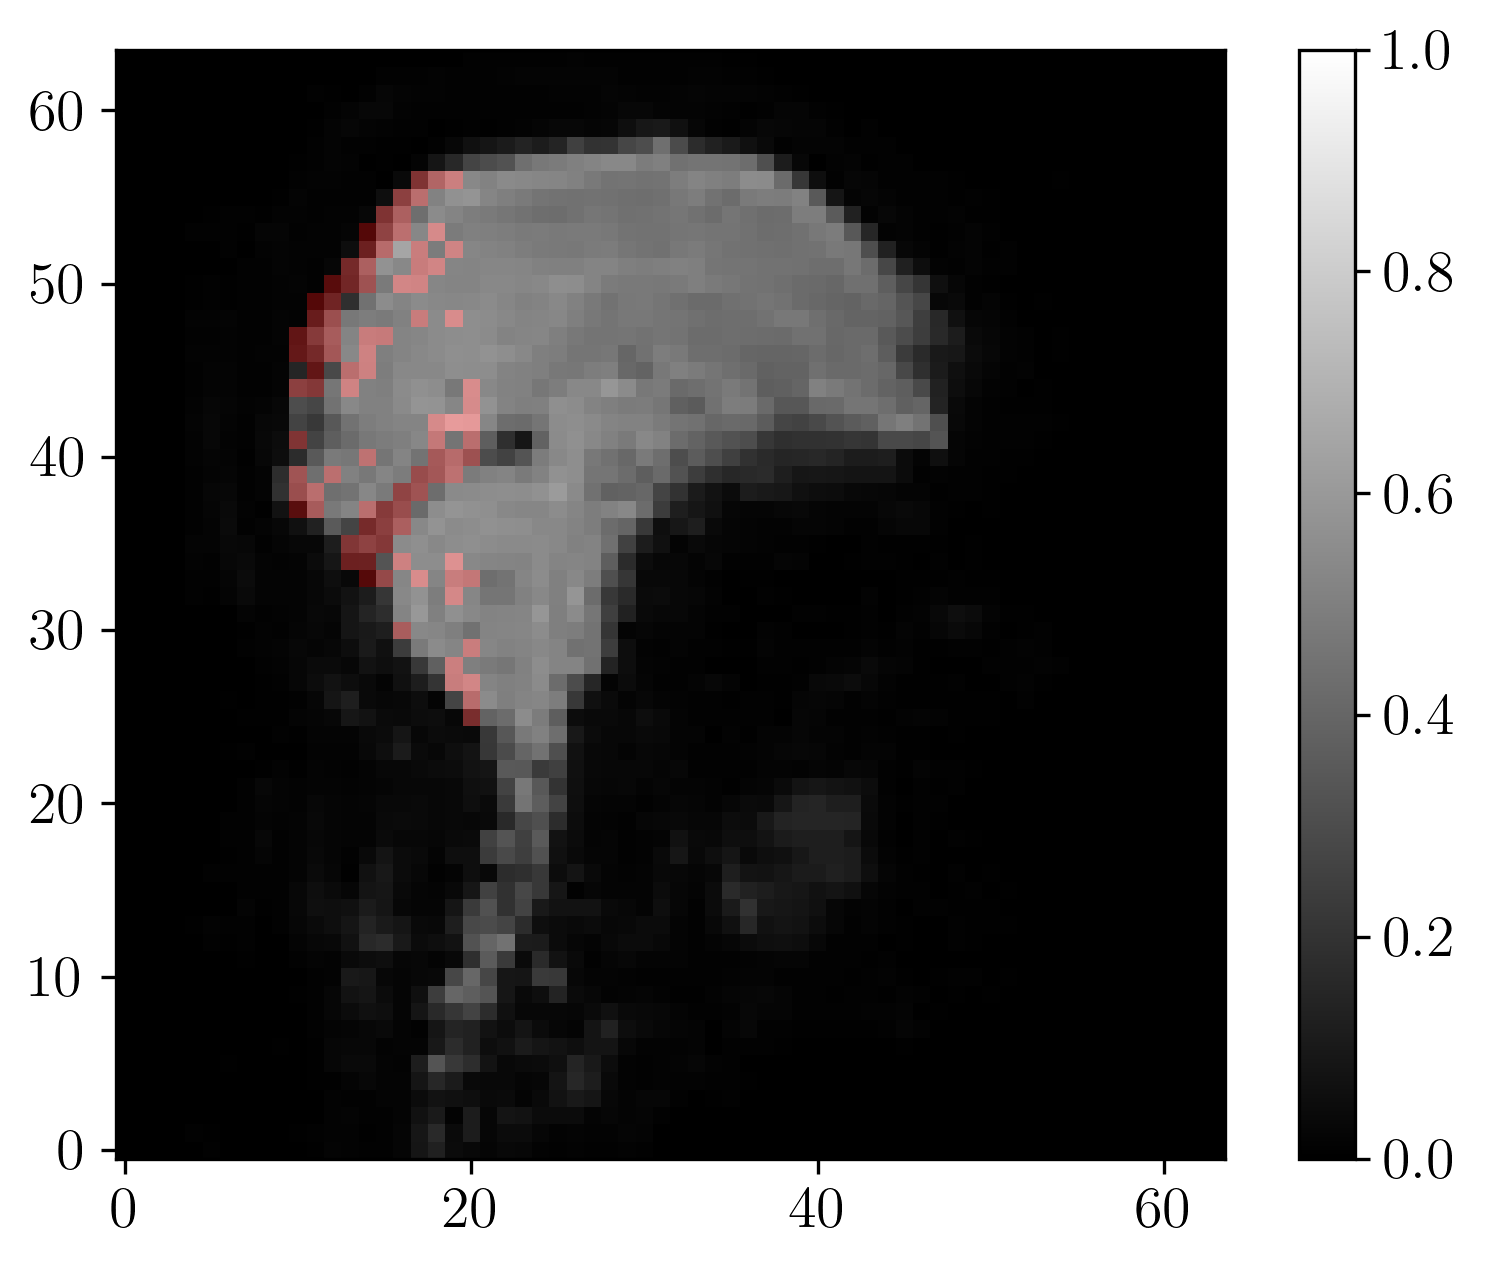
\includegraphics[width=0.33\textwidth]{local/sub-47-5-1-1000-37-20-_-_-test.png}}}
	\hfill
	\subfloat[Predicted]{\label{fig:local-b}{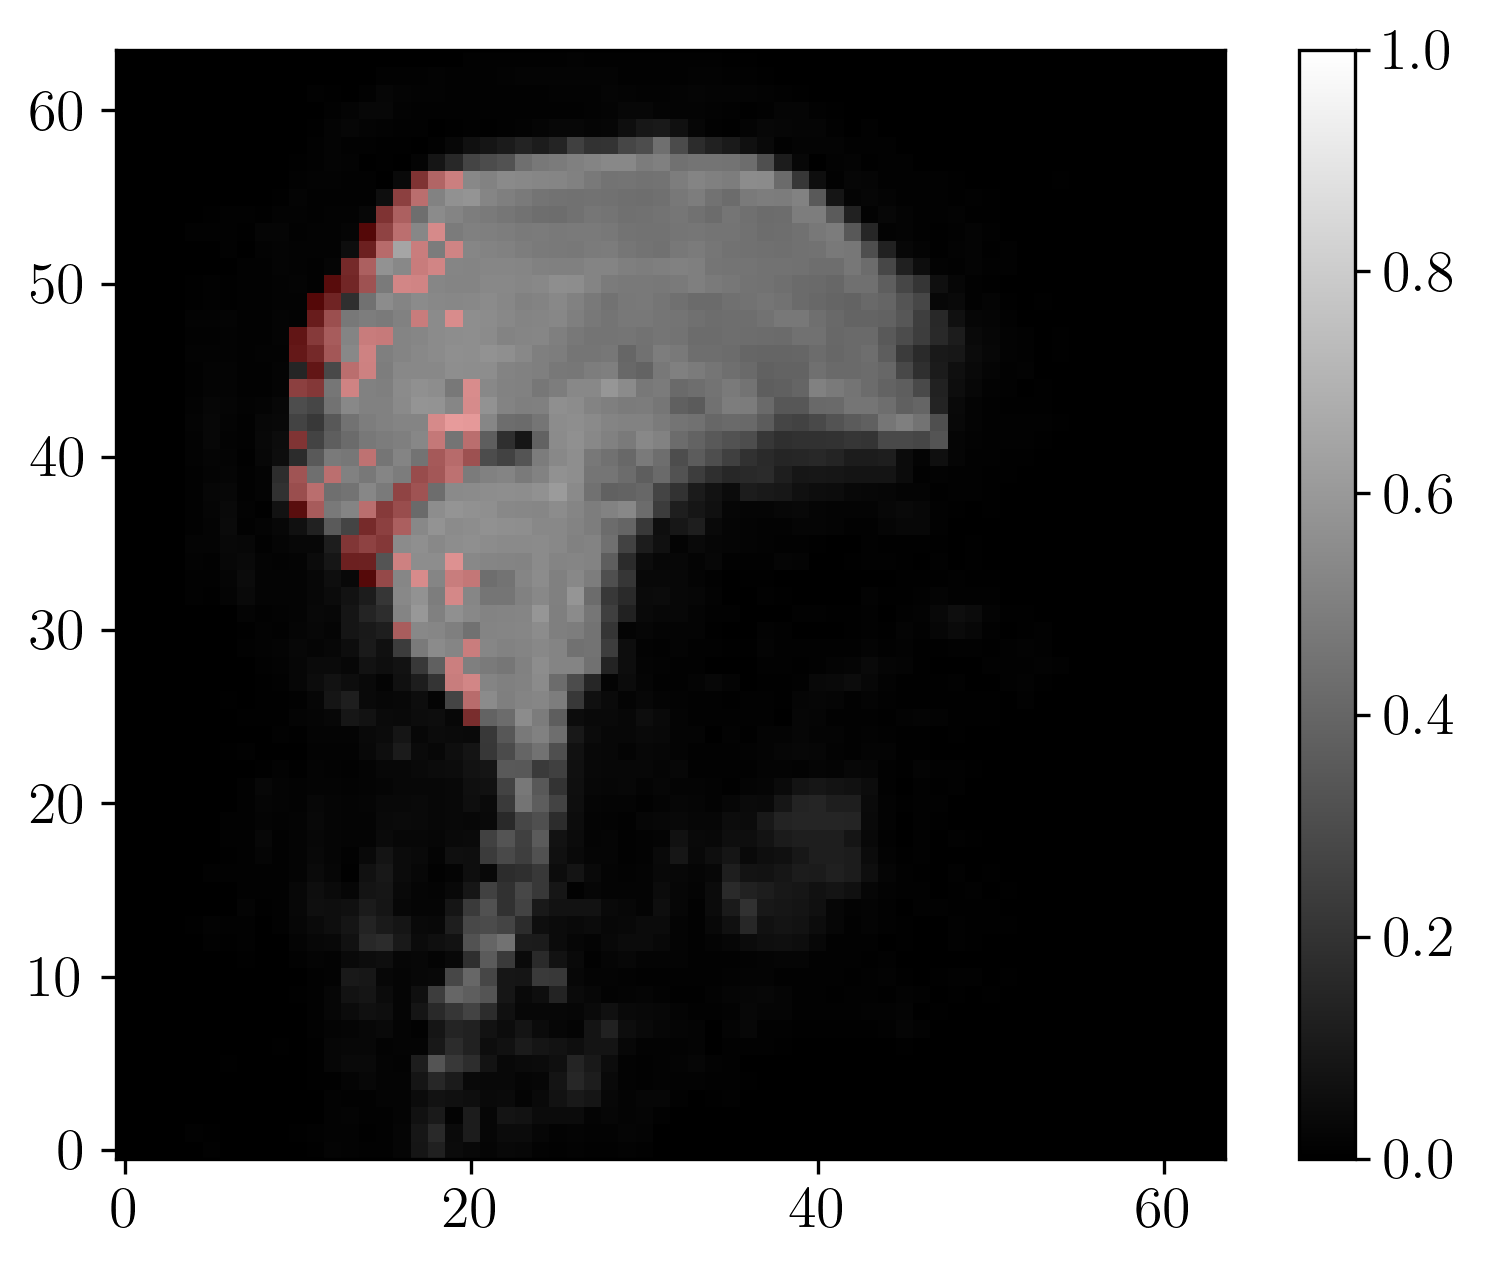
\includegraphics[width=0.33\textwidth]{local/sub-47-5-1-1000-37-20-_-_-predicted.png}}}
	\hfill
	\subfloat[Difference]{\label{fig:local-c}{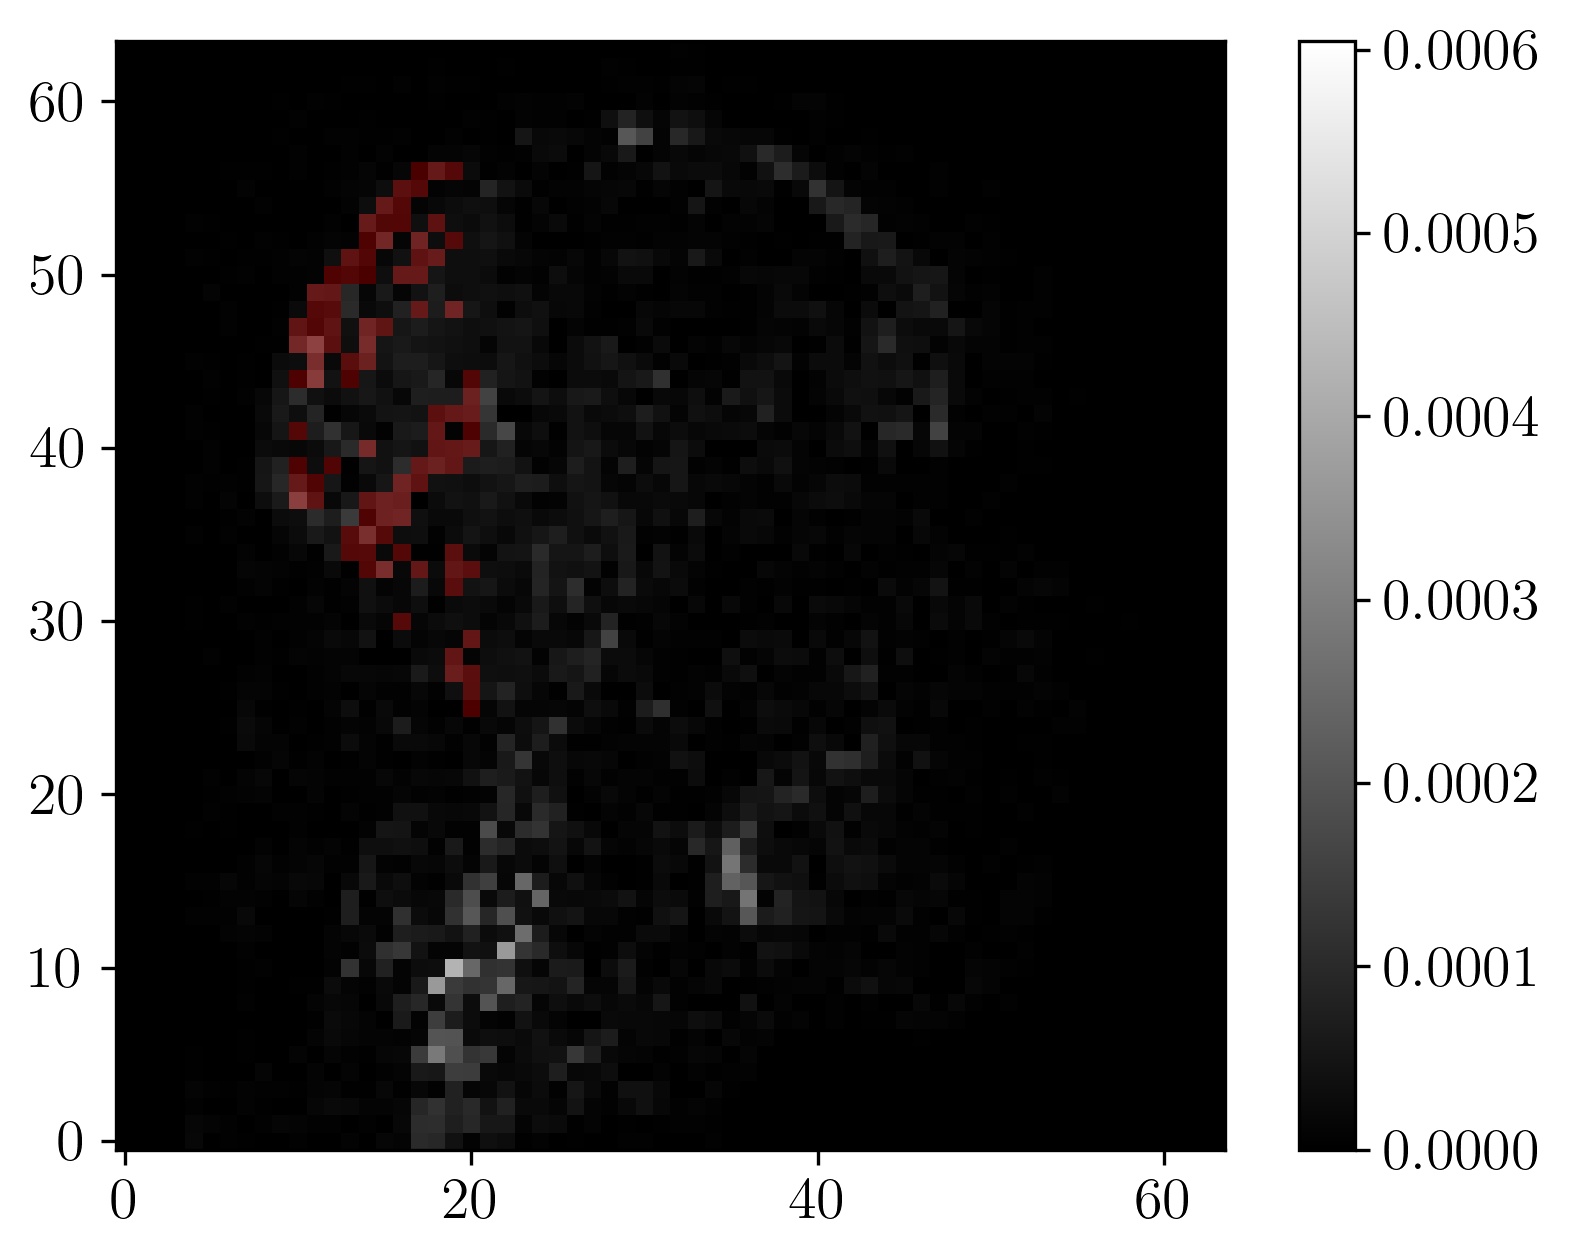
\includegraphics[width=0.33\textwidth]{local/sub-47-5-1-1000-37-20-_-_-difference.png}}}
	\caption{Localization of the most active zone}
	\label{fig:local}
\end{figure}

\begin{figure}[h!]
	\centering
	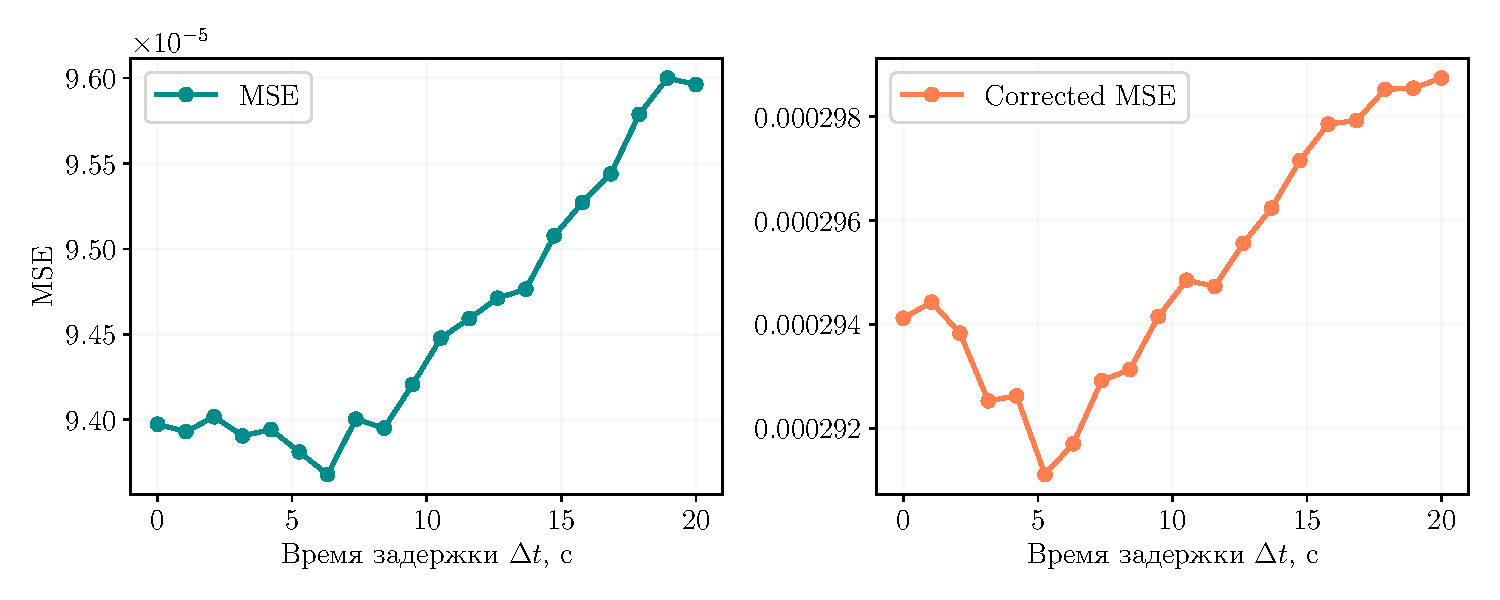
\includegraphics[width=\textwidth]{mse_dt.pdf}
	\caption{Dependence of MSE on delay time}
	\label{fig:mse-dt}
\end{figure}

\paragraph*{Optimal regularization parameter.}

The dependence of MSE on the regularization parameter $\alpha$ was analyzed.
Compression factors 1, 2, 4, and 8 were considered.
The corresponding graphs are shown in Figure~\ref{fig:mse-alpha}.
Averaging over the subjects was performed to construct the graph.
The limits of standard deviation are marked.
The graphs show that the optimal value of the coefficient $\alpha \approx 1000$.
The curve shape is preserved regardless of the compression factor of fMRI images.

\begin{figure}[h!]
	\centering
	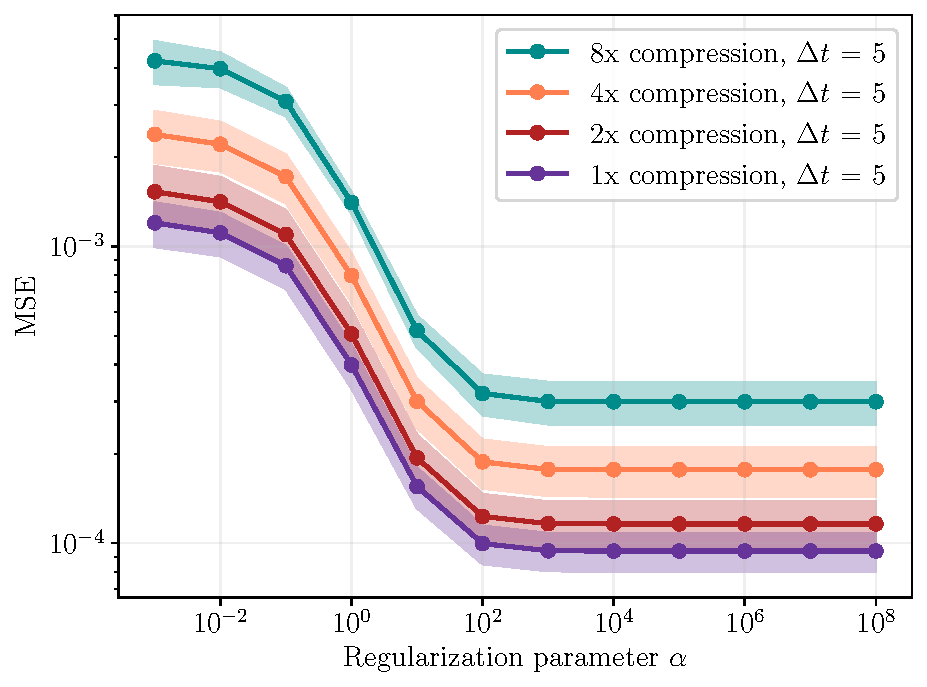
\includegraphics[width=0.65\textwidth]{subs_MSE_alpha.pdf}
	\caption{Dependence of MSE metric on regularization parameter $\alpha$ on images from the test sample}
	\label{fig:mse-alpha}
\end{figure}

\paragraph*{Effect of image compression ratio on method runtime.}

We compare the training time of the model when using different
compression coefficients of fMRI images. Coefficients 1, 2, 4 and 8 are considered.
For each value of the compression ratio, the average value of the model training time for all subjects is calculated.
value of the model training time. The standard deviation is calculated.
The experimental results are summarized in Table~\ref{table:coeffs}.
The running time of the method is significantly reduced when using
pre-compression of fMRI images. 
The experiment with the selection of the optimal regularization coefficient
confirms that the compression of the images does not change the dependences.

\begin{table}[h!]
	\centering
	\caption{Dependence of model training time on compression ratio}
	\begin{tabular}{|c|c|c|}
		\hline
		Compression coefficient & Mean time, s & Std, s \\ \hline \hline
		1 & 36.3 & 6.1 \\ \hline
		2 & 6.7 & 0.5 \\ \hline
		4 & 1.6 & 0.1 \\ \hline
		8 & 1.4 & 0.3 \\ \hline
	\end{tabular}
	\label{table:coeffs}
\end{table}

\paragraph*{Analyzing the distribution of model weights.}

A graph of the distribution of the values of the components of the model weight vector was plotted.
To construct it, we averaged over all voxels for the 4th subject.
The result is shown in Figure~\ref{fig:w-distr}.
The model weights do not lie in the neighborhood of any particular value, 
that is, their distribution is not degenerate.
This result is quite consistent with reality, because a human being, while viewing
pays attention to certain parts of the frame, such as characters or other details.
other details.

\begin{figure}[h!]
	\centering
	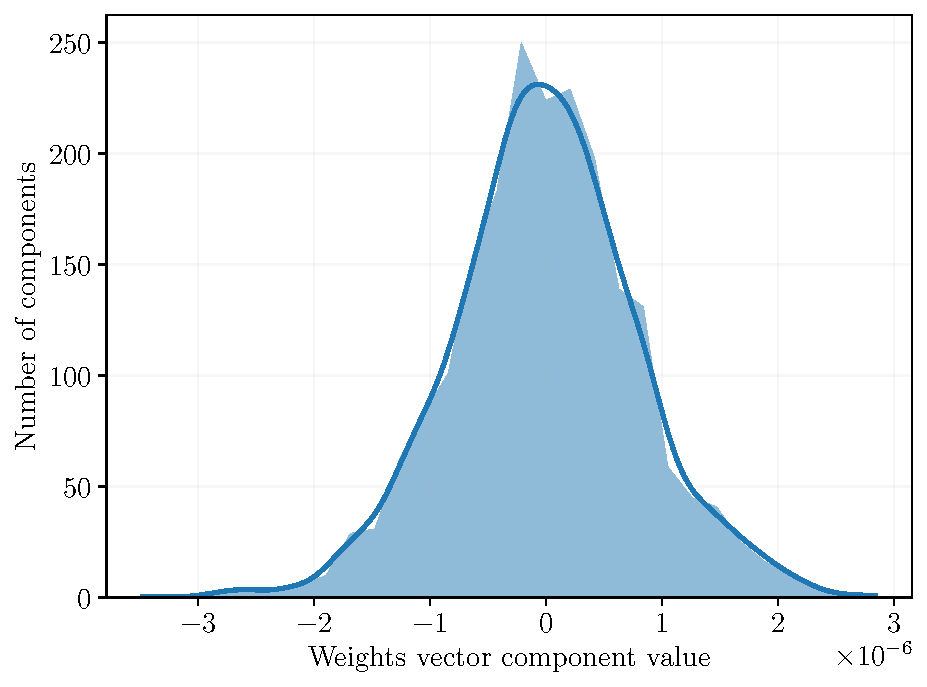
\includegraphics[width=0.65\textwidth]{distribution.pdf}
	\caption{Weights vector component distribution}
	\label{fig:w-distr}
\end{figure}

\paragraph*{Hypothesis of invariance of model weights with respect to humans.}

The hypothesis of invariance of the model weights with respect to the person was tested:
Using one subject's weight matrix to reconstruct another subject's fMRI images.
The MSE metric on the test sample was used.
The results are presented in Table~\ref{table:inv}.
The 4th and 7th subjects were considered. The weight matrix of the 4th was used to reconstruct the
of the 7th subject's images.
The MSE values are almost the same.

\begin{table}[h!]
	\centering
	\caption{Testing the hypothesis of invariance of model weights with respect to humans}
	\begin{tabular}{|c|c|c|c|}
		\hline
		Weights matrix & True             & Mixed  & Difference        \\ \hline \hline
		MSE           & $9.7494 \cdot 10^{-5}$ & $9.7498 \cdot 10^{-5}$ & $3.96 \cdot 10^{-9}$ \\ \hline
	\end{tabular}
	\label{table:inv}
\end{table}

A similar experiment was conducted for each pair of subjects.
The obtained results are presented in Figure~\ref{fig:heatmap},
which was obtained as follows.
Some subject (corresponding to a row of the matrix) is considered, 
MSE~--- <<true>> is calculate.d for him.
Next, another subject is considered (corresponding to a column of the matrix),
its matrix of weights is taken, and a prediction is made for the first 
subject, then the MSE~--- <<subtracted>> is calculated. 
The difference between the resulting MSE as a percentage of the <<true>> is entered into the matrix.
A positive value means that the <<mixed>> MSE is greater than the <<true>>.
A negative~--- that the <<substituted>> is smaller.
That is, there is a MAPE on the heatmap.
The ideal model should result in only positive deviation values, however,
as can be seen in Figure~\ref{fig:heatmap}, there are negative values in the matrix.
Nevertheless, they are rather small, namely, they correspond to deviations of the order of 1\%.
This is explained by the fact that the model is quite simple, and therefore has a
high generalizing ability.
However, this does not prevent us from concluding that the data do not contradict the hypothesis 
about the invariance of the model weights with respect to humans.

\begin{figure}[h!]
	\centering
	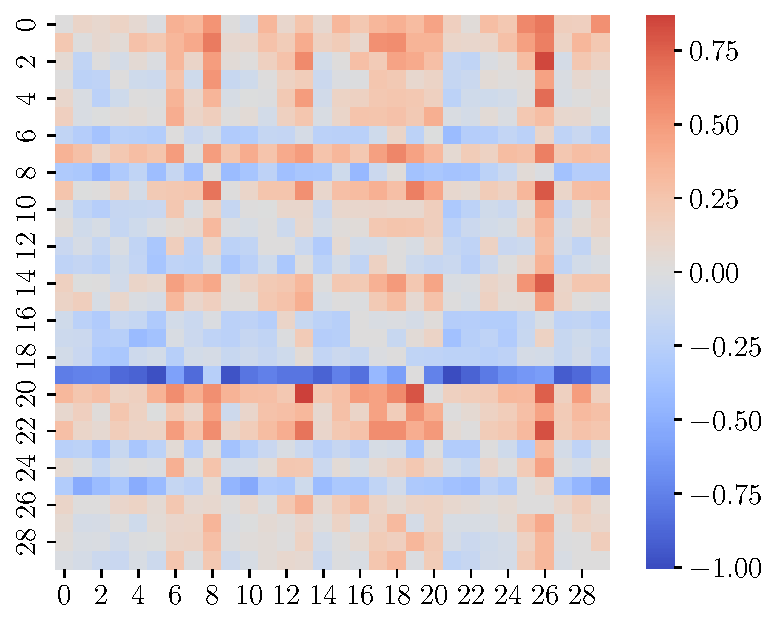
\includegraphics[width=0.5\textwidth]{heatmap.pdf}
	\caption{MAPE of MSE changing when predicting on the mixed weight matrix}
	\label{fig:heatmap}
\end{figure}

\paragraph*{Method corectness.}

The quality of the method performance on uninformative data is considered.
A matrix consisting entirely of units was taken as a matrix of objects-signs $\bX$.
Comparison with the results on the present feature-description matrix was made.
To the first snapshot of the 35th subject, all the reconstructed
changes in voxel values.
As a result, we have the last snapshot of the sequence. Figure~\ref{fig:recover}
are slices of the last true and recovered snapshots from the test sample.
Figure\myfigref{fig:recover}{fig:recover-c} shows the difference between them.
The results on the uninformative ones are demonstrated in Figure~\ref{fig:random}.
The difference between the true and recovered images when working with uninformative data
is much higher, which confirms that there is a correlation between the sensor readings and the
images from the video sequence. The numerical results are summarized in Table~\ref{table:random}.

\begin{figure}[h!]
	\centering
	\subfloat[True]{\label{fig:recover-a}{\includegraphics[width=0.33\textwidth]{original/sub-35-5-1-1000--1-20-_-_-recovered-test.png}}}
	\hfill
	\subfloat[Predicted]{\label{fig:recover-b}{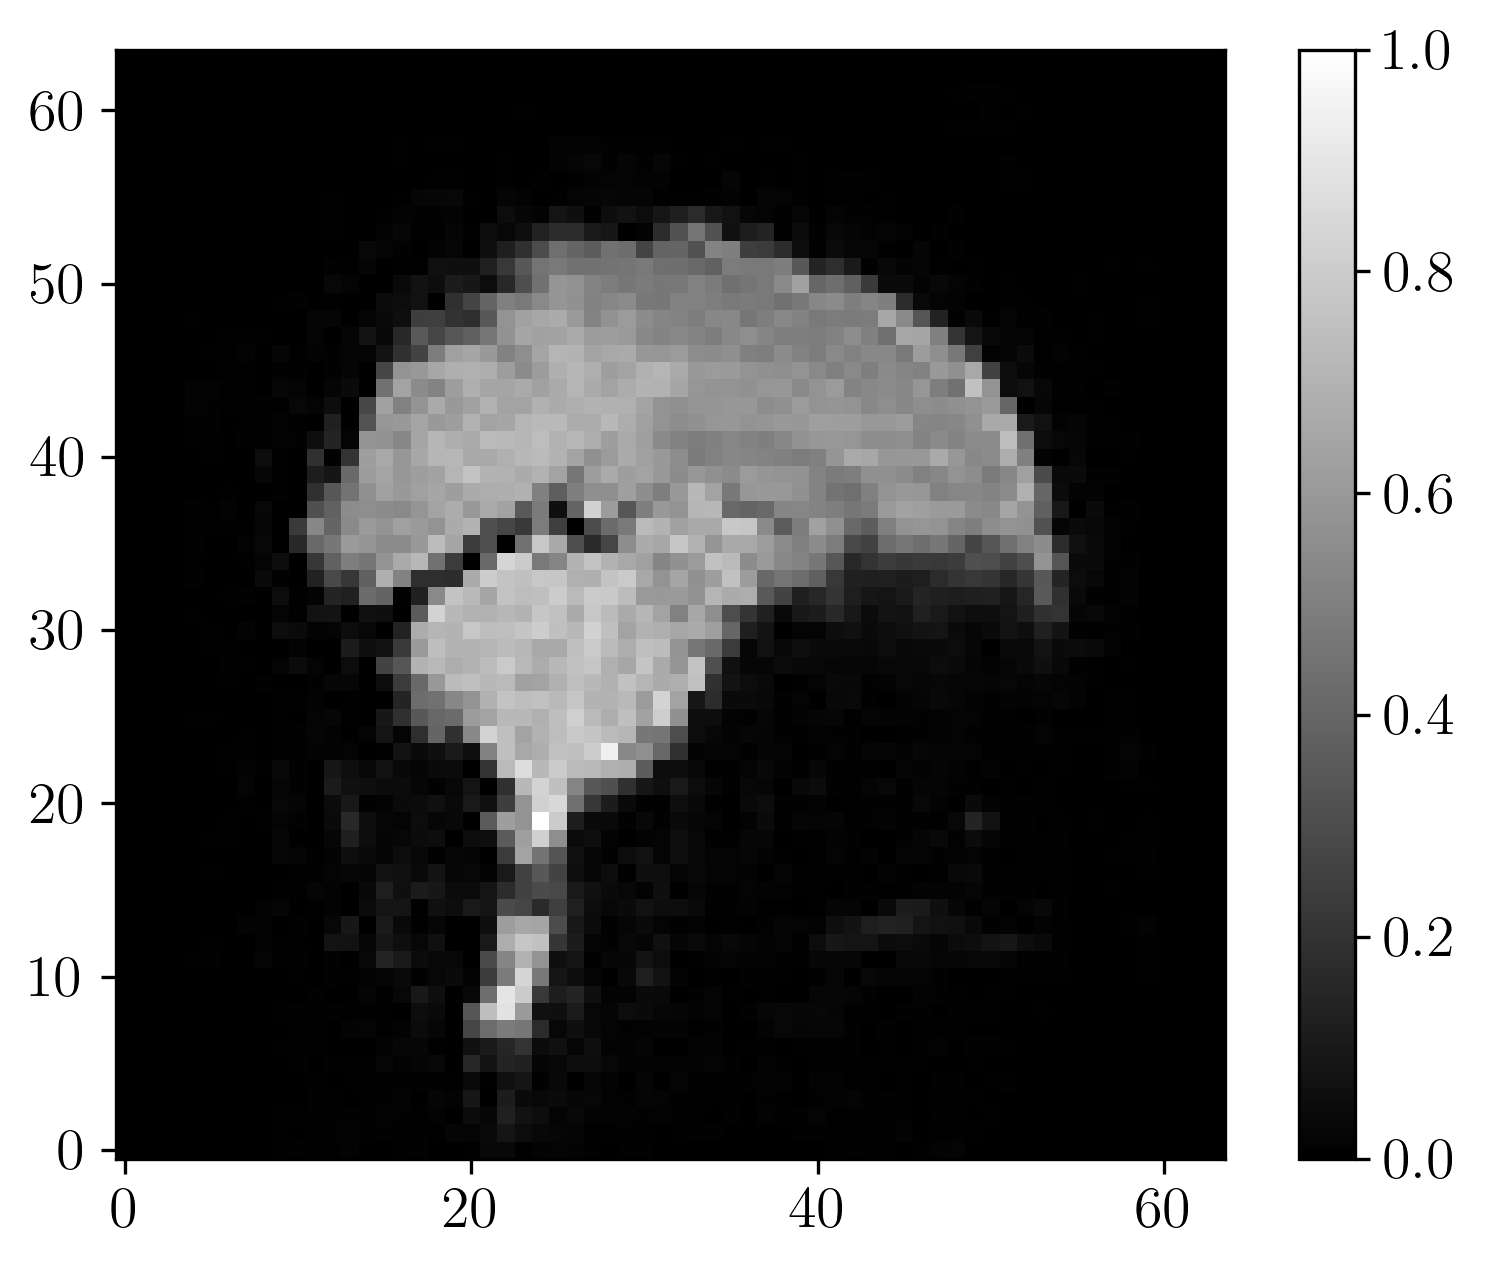
\includegraphics[width=0.33\textwidth]{original/sub-35-5-1-1000--1-20-_-_-recovered-predicted.png}}}
	\hfill
	\subfloat[Difference]{\label{fig:recover-c}{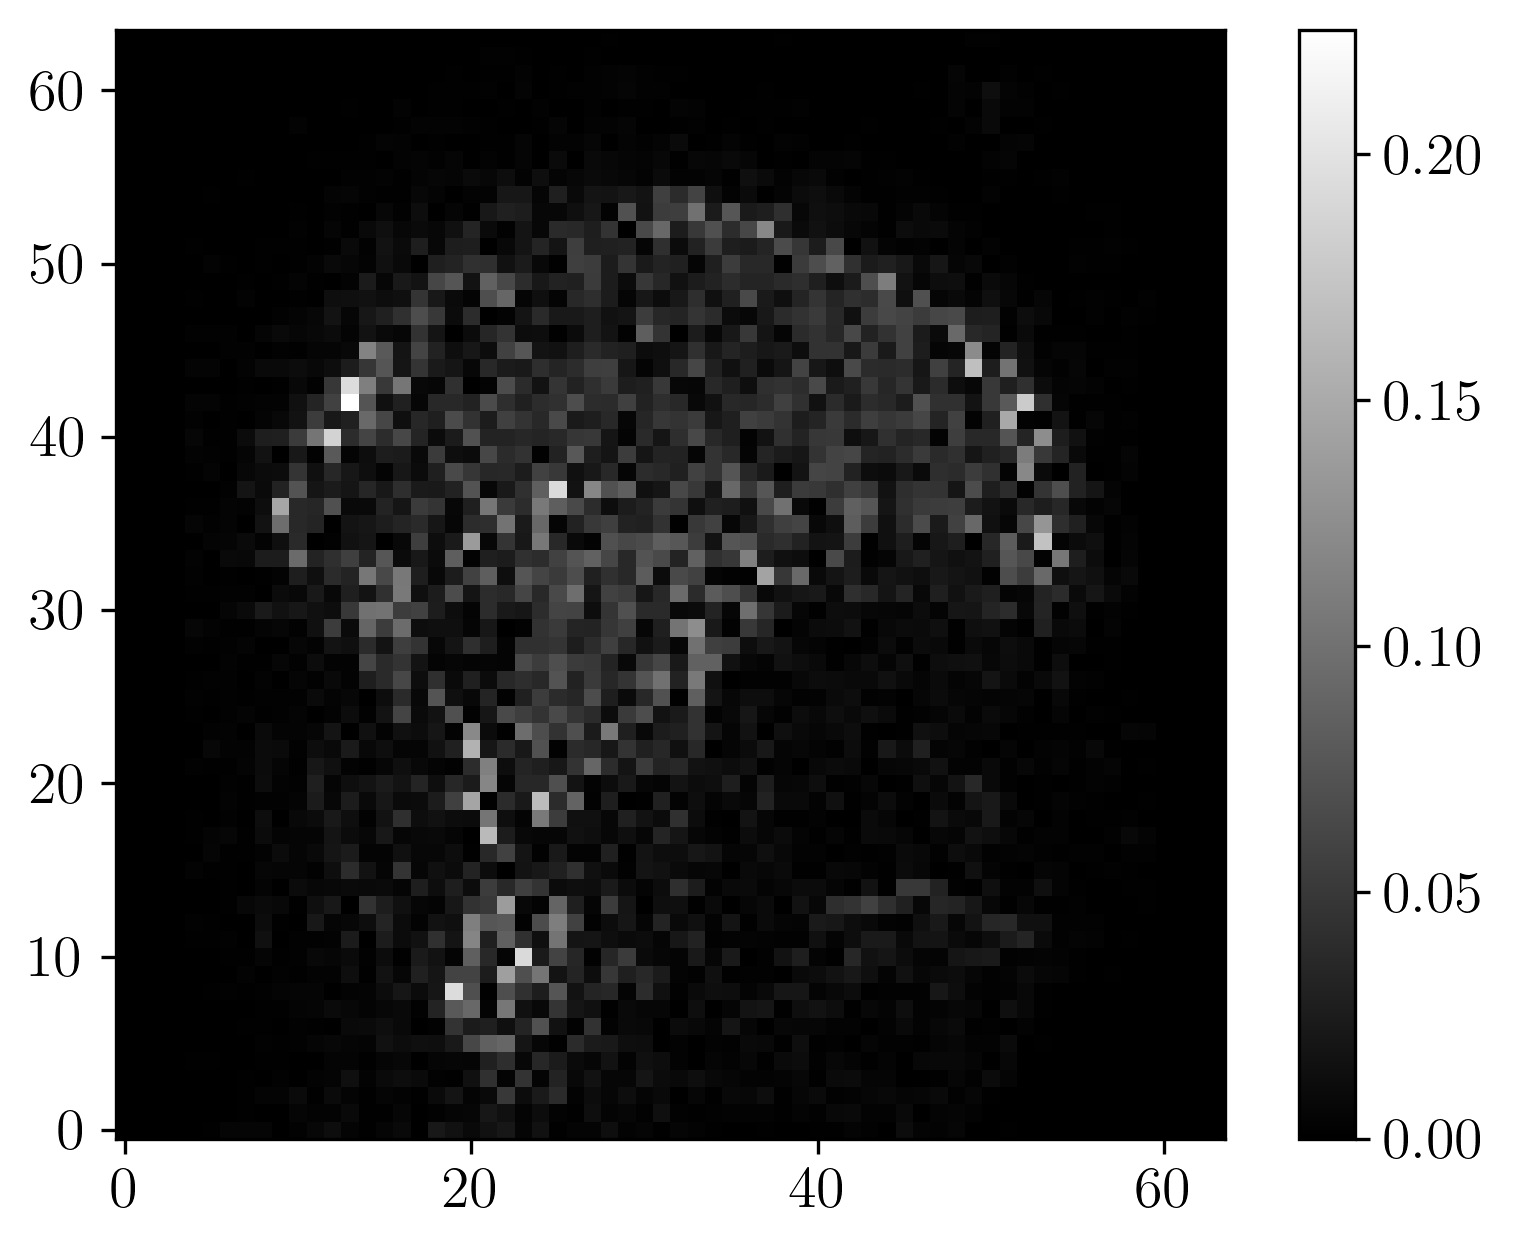
\includegraphics[width=0.33\textwidth]{original/sub-35-5-1-1000--1-20-_-_-recovered-difference.png}}}
	\caption{Slices of fMRI images from the test sample}
	\label{fig:recover}
\end{figure}

\begin{figure}[h!]
	\centering
	\subfloat[True]{\label{fig:random-a}{\includegraphics[width=0.33\textwidth]{noised/sub-35-5-1-1000--1-20-_-_-recovered-test.png}}}
	\hfill
	\subfloat[Predicted]{\label{fig:random-b}{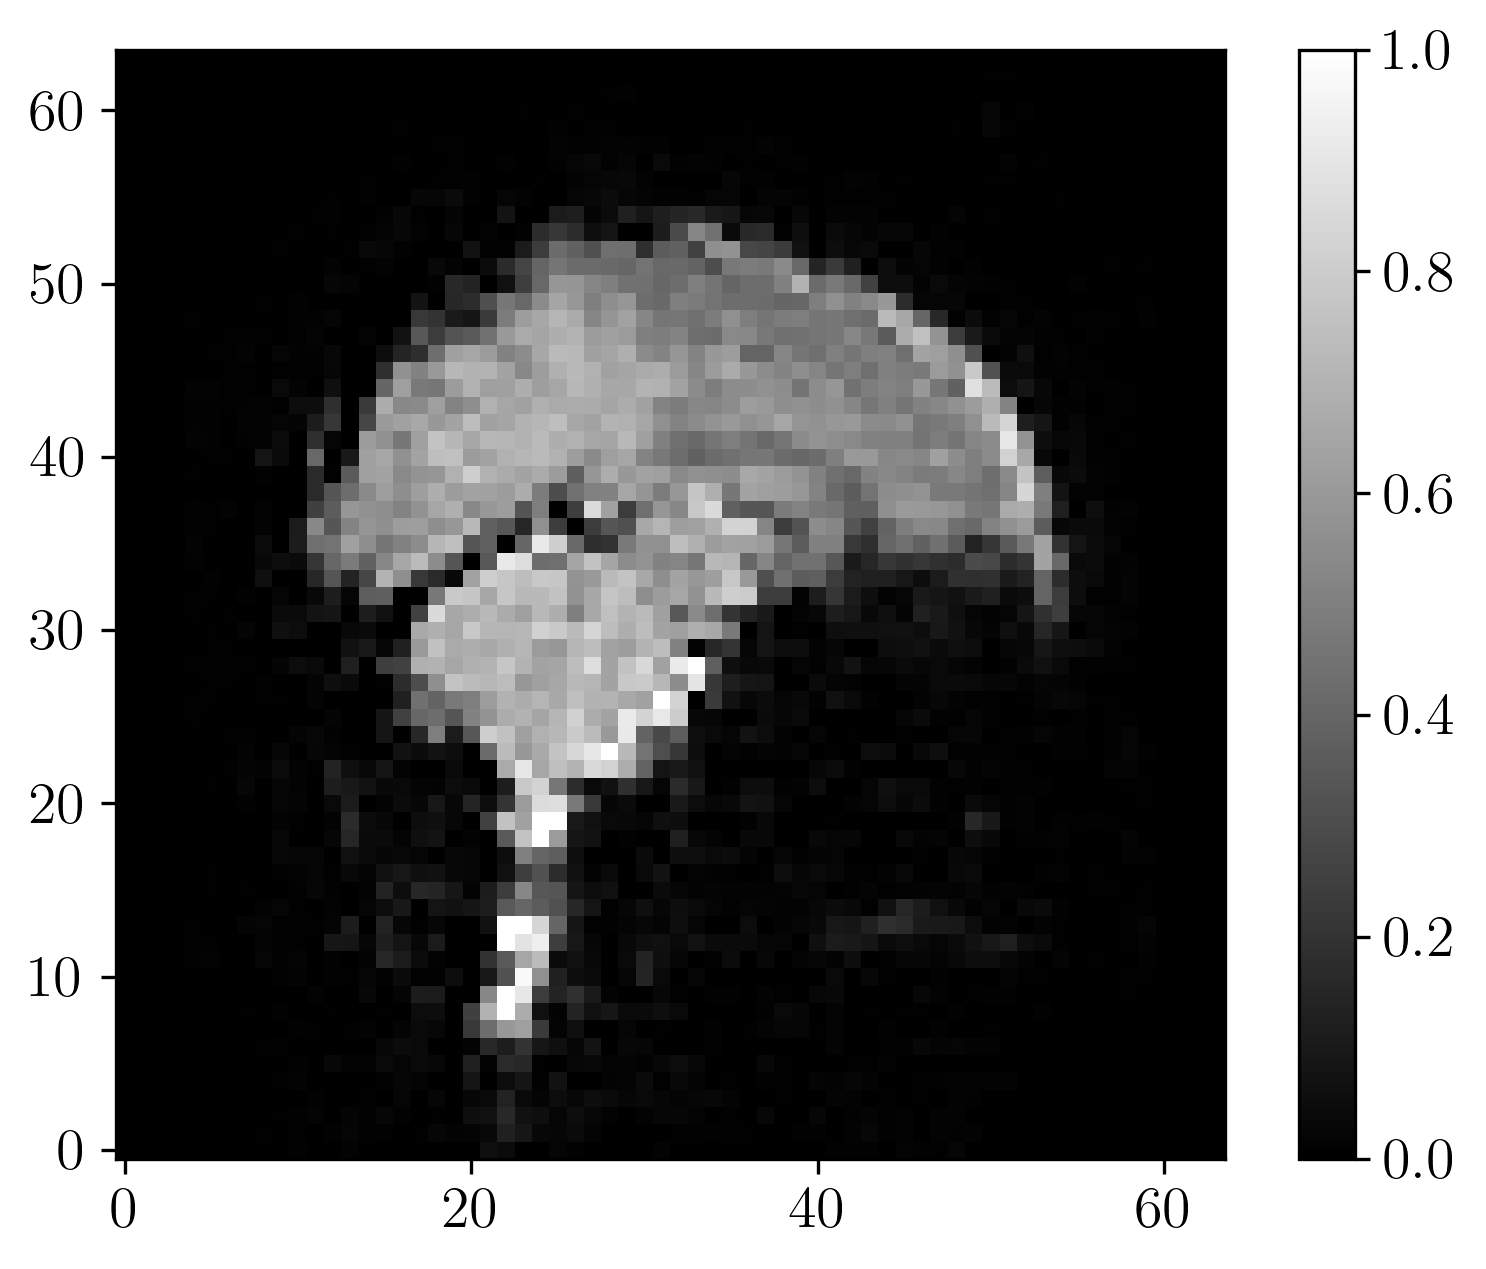
\includegraphics[width=0.33\textwidth]{noised/sub-35-5-1-1000--1-20-_-_-recovered-predicted.png}}}
	\hfill
	\subfloat[Difference]{\label{fig:random-c}{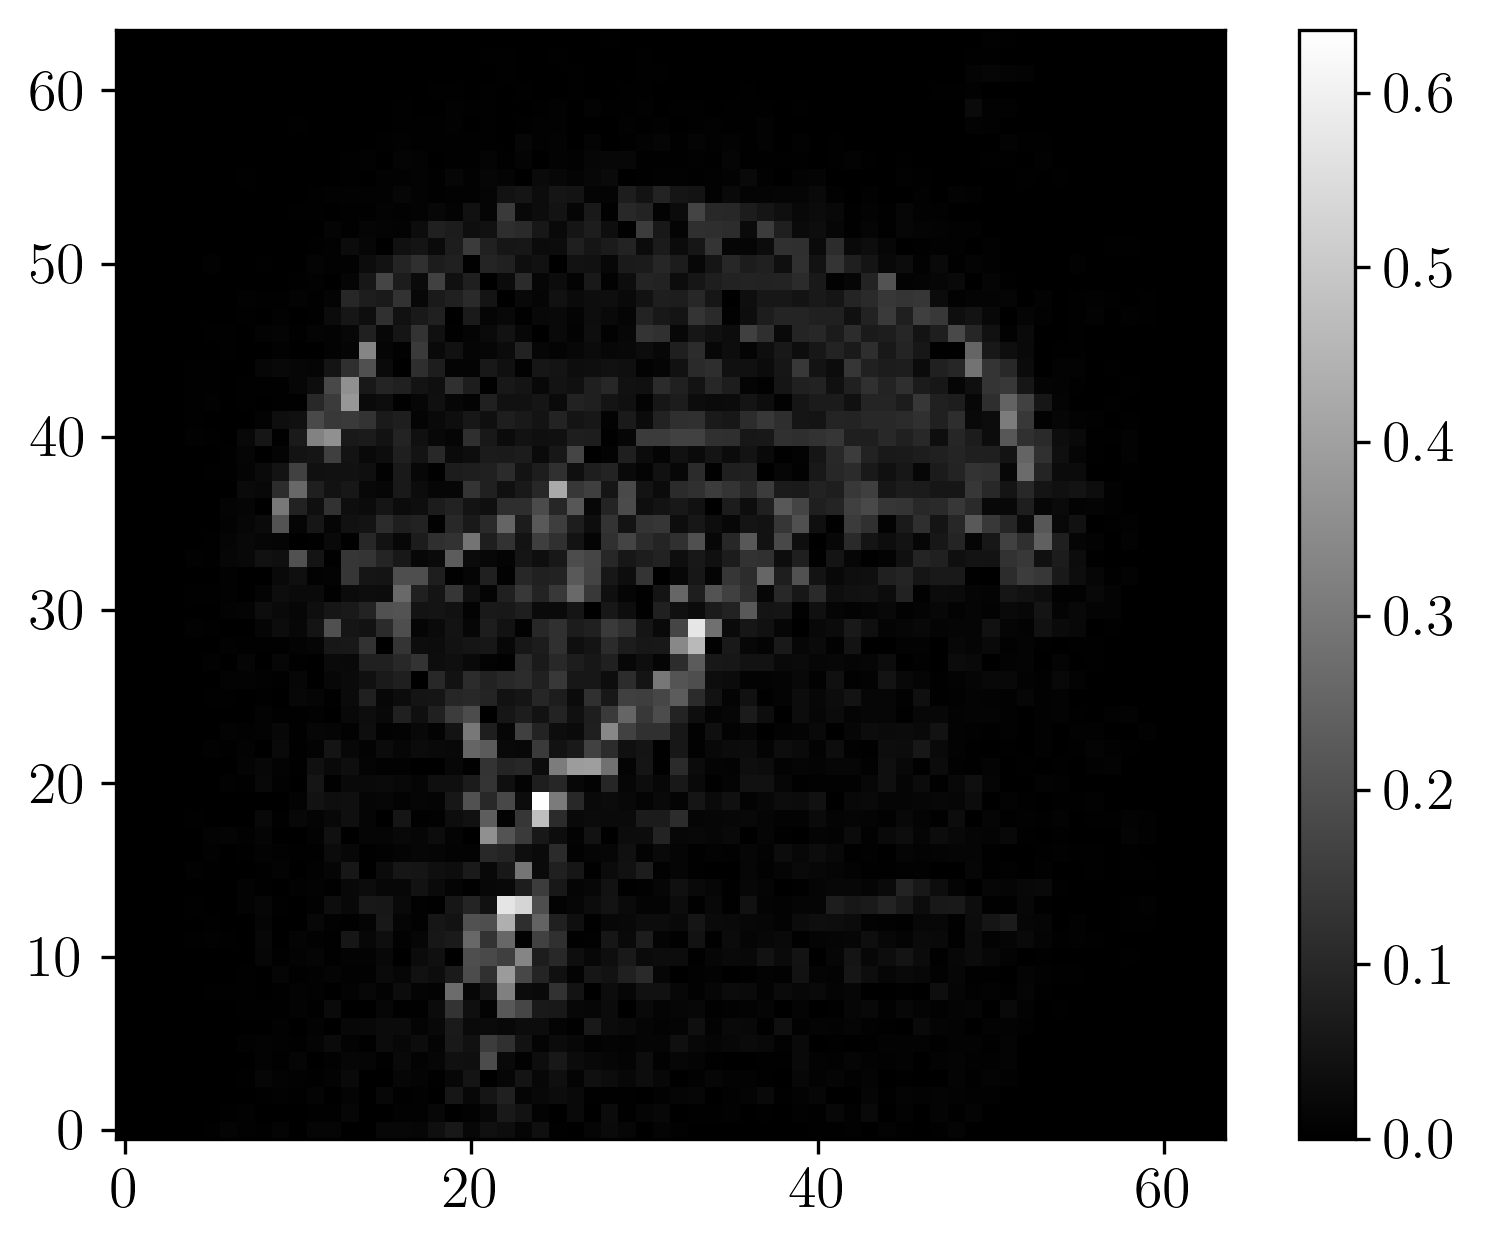
\includegraphics[width=0.33\textwidth]{noised/sub-35-5-1-1000--1-20-_-_-recovered-difference.png}}}
	\caption{Slices of fMRI images from the test sample (uninformative data)}
	\label{fig:random}
\end{figure}

\begin{table}[h!]
	\centering
	\caption{Quality of method performance on uninformative data}
	\begin{tabular}{|c|c|c|c|}
		\hline
		Data & True          & Uninformative & Difference \\ \hline \hline
		MSE     & $4.87 \cdot 10^{-4}$ & $1.76 \cdot 10^{-3}$ & $1.27 \cdot 10^{-3}$ \\ \hline
	\end{tabular}
	\label{table:random}
\end{table}


\paragraph*{Correlation data analysis.}

Let us carry out an additional study of the data presented in the sample \citep{Berezutskaya2022}.
As mentioned earlier, the dataset also contains information about the time of appearance
and disappearance of individual objects in the frame. We use this information to compose a feature-based
description of the images of the video sequence of lower dimensionality. In total, there is information about 135 different objects.
Let's encode each image with a vector of 0 and 1 of dimension 135, where 0 corresponds to the absence of an object in the frame and 1~ to the absence of an object in the frame.
object in the frame, and 1~--- its presence.

The object that most often appears and disappears from the frame~--- Pippi, the main character in the movie shown to the subjects. 
The number of different fragments where she is in the frame is 26. We investigate the cross-correlation of the time series corresponding to this object with the 
with the time series of fMRI images.

\begin{figure}[h!]
	\centering
	\subfloat[True]{\label{fig:occur-a}{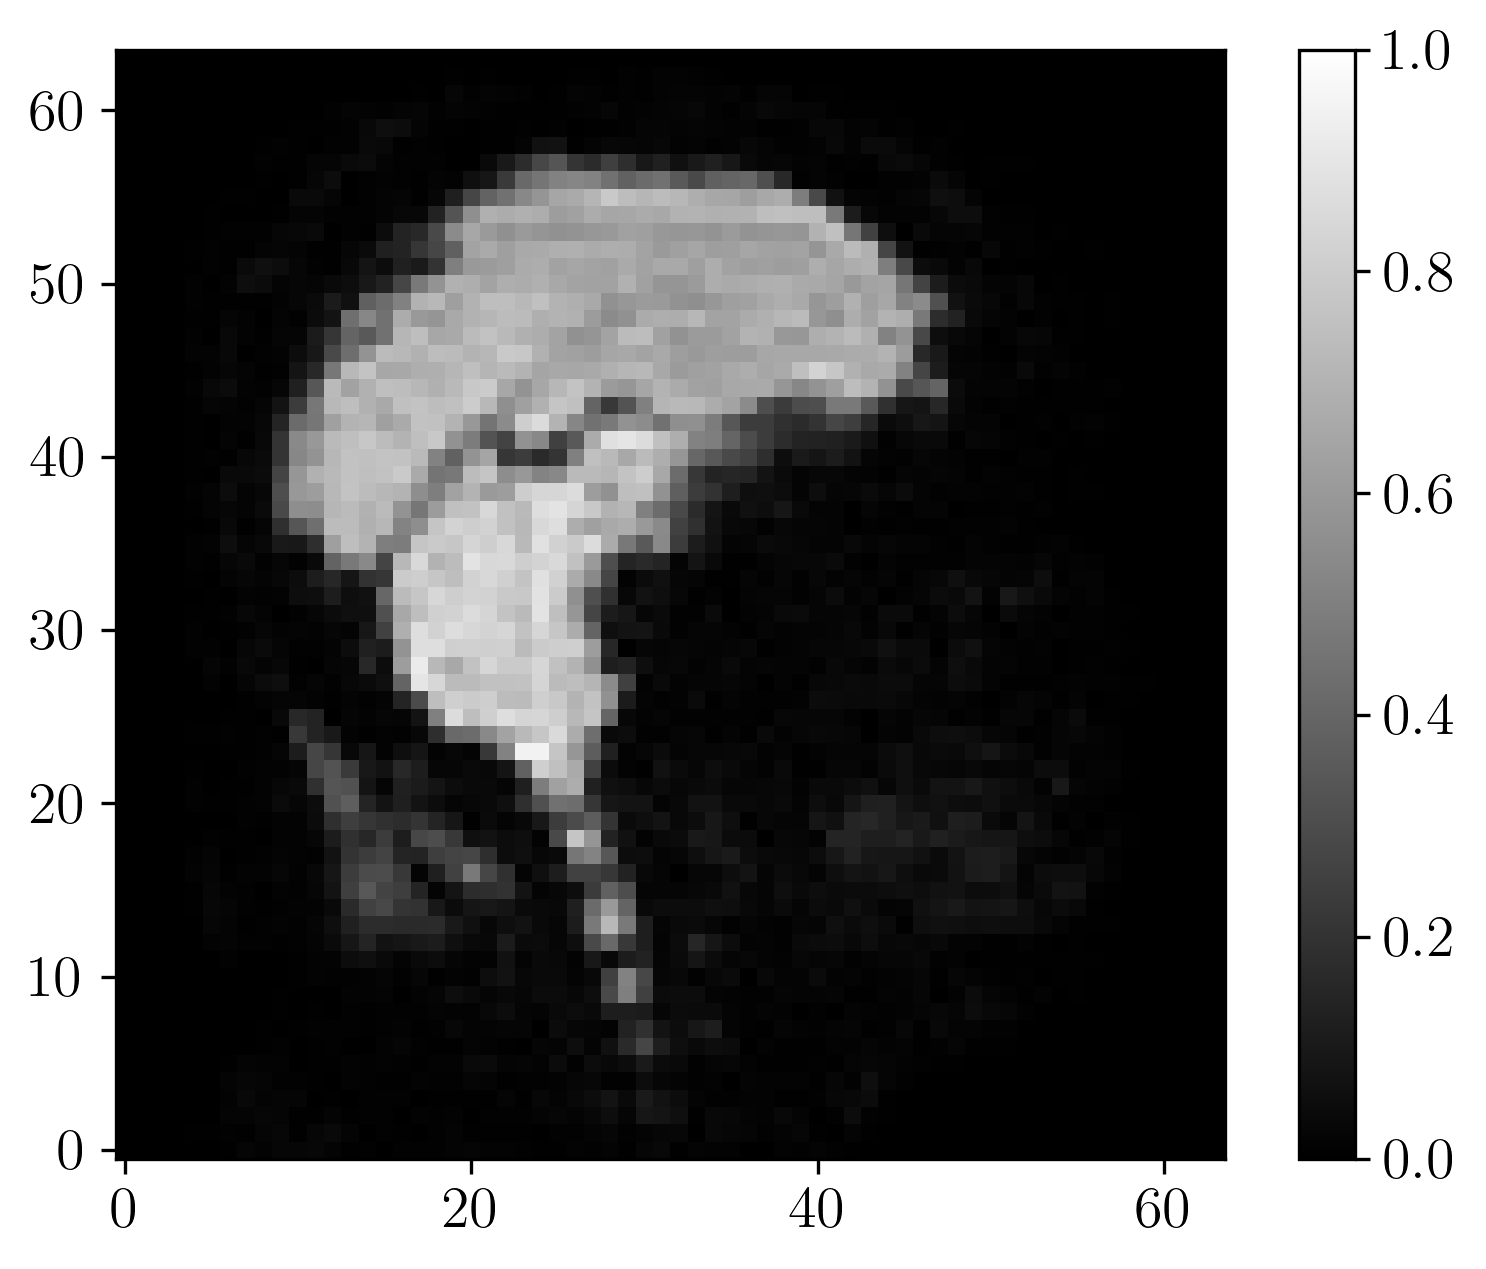
\includegraphics[width=0.33\textwidth]{scan_test.png}}}
	\hfill
	\subfloat[By cross-correlation]{\label{fig:occur-b}{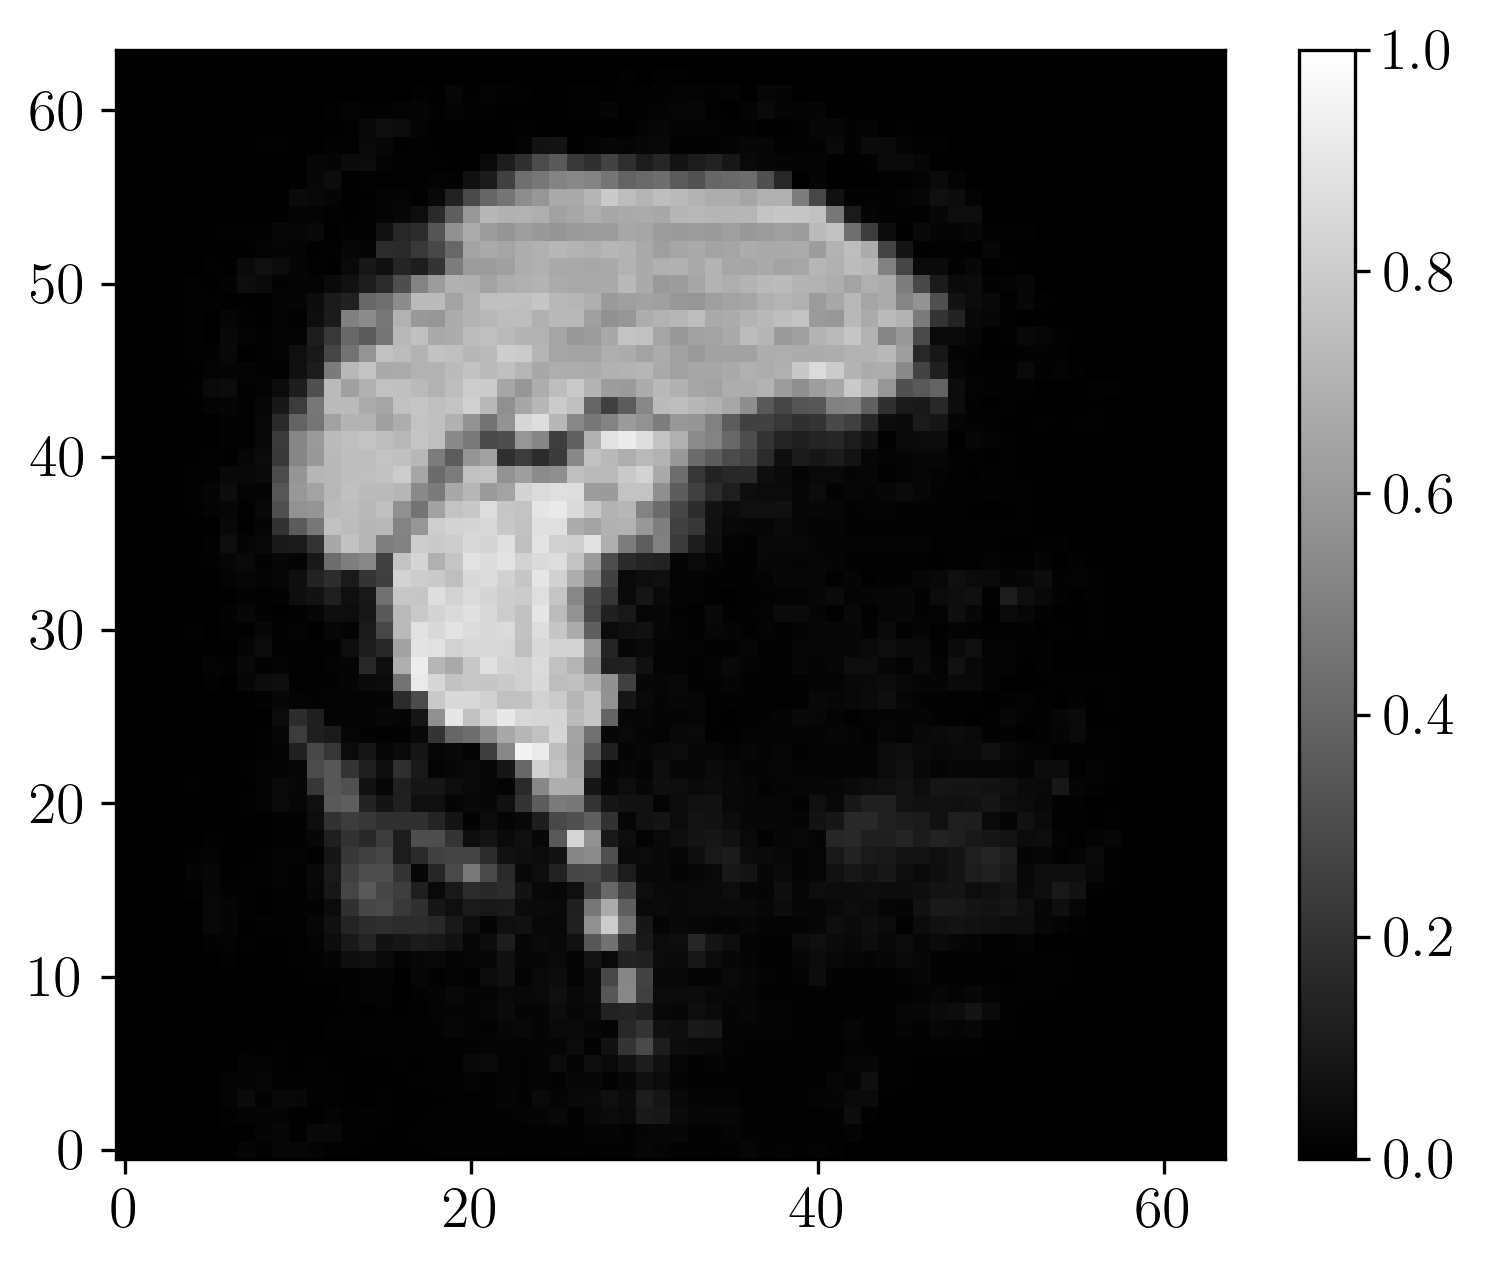
\includegraphics[width=0.33\textwidth]{scan_cross_correlation.png}}}
	\hfill
	\subfloat[Difference]{\label{fig:occur-c}{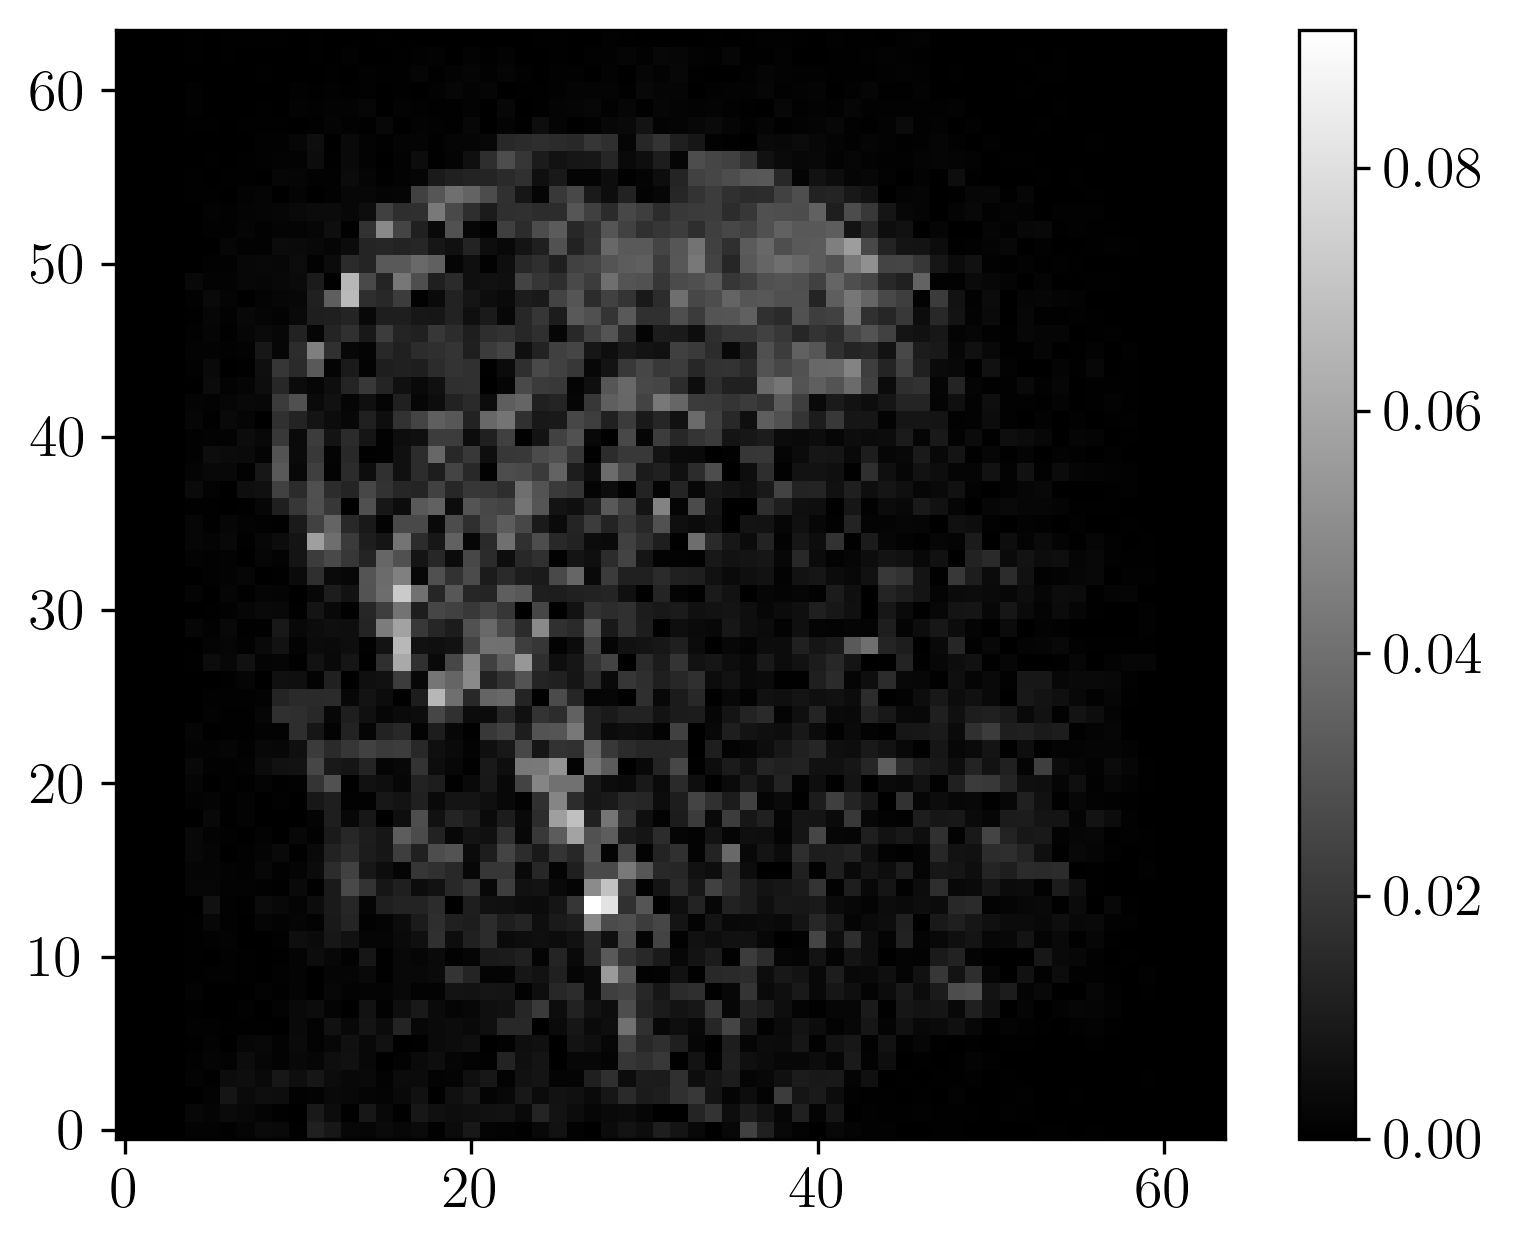
\includegraphics[width=0.33\textwidth]{scan_difference.png}}}
	\caption{Slices of fMRI images from the test sample (compared to cross-correlation)}
	\label{fig:occur}
\end{figure}

Figure\myfigref{fig:occur}{fig:occur-a} shows a real fMRI image from the test sample. 
The 7th subject was selected, and the 20th slice on the first coordinate of the 37th image in the sequence.
Figure\myfigref{fig:occur}{fig:occur-b} presents the snapshot that was obtained from the cross-correlation function values.
Namely, for each voxel, a time series corresponding to its change over time was obtained.
Next, its cross-correlation function with the selected object was computed.
Then, an offset was selected that corresponds to a delay time on the order of 5 seconds.
The obtained number for each voxel was normalized to the segment $[0; 1]$.

As can be seen from Figure\myfigref{fig:occur}{fig:occur-c}, the images are almost identical. 
The MSE value is $7.8 \cdot 10^{-5}$. This further confirms the fact that the human brain reacts 
to the appearance and disappearance of specific objects in the frame.

\section{Conclusion}

In this paper we consider the task of restoring the dependence between the readings
fMRI sensors and human perception of the external world.
The method of approximation of fMRI images sequence by video sequence is proposed. 
The method takes into account the hemodynamic response time~--- the delay time between the images from the video sequence and the fMRI images. 
A linear model is independently constructed for each voxel of the fMRI image. 
Each linear model is constructed under the assumption that the sequence of fMRI images is Markovian. 
In the experiments, the optimal value of the delay time is selected for each subject. 
The optimal value is found from analyzing the plot of MSE versus delay time.
The regularization coefficient is selected. 
The effect of fMRI image compression ratio on model training time is investigated.
It is assumed that the occipital lobe of the brain is responsible for information from visual organs.
MSE correction is performed based on localization of this region and selection of the most changing voxels. 
With this construction, the graph has a characteristic minimum corresponding to the optimal value of the delay time.
The obtained value of the delay time is consistent with neurobiological information.
The experimental MSE values are small, indicating that there is a correlation between the data. 
The variation of images in the video sequence is taken into account since the distribution of model weights is not degenerate.
The hypothesis of invariance of model weights with respect to humans is tested. 
The correctness of the method is confirmed by experiments with random data.

\bibliographystyle{unsrtnat}
\bibliography{fMRI_2023.bib}

\end{document}